\documentclass[conference]{IEEEtran}

% ─── Packages ────────────────────────────────────────────────────────────────
\usepackage[T1]{fontenc}
\usepackage[utf8]{inputenc}
\usepackage{graphicx}
\usepackage{amsmath}
\usepackage{booktabs}
\usepackage{tabularx}
\usepackage{listings}
\usepackage{xcolor}
\usepackage{hyperref}
\usepackage{float}
\usepackage{microtype}
\usepackage{array}
\usepackage{caption}

% ─── Code listing style ───────────────────────────────────────────────────────
\definecolor{codebg}{rgb}{0.96,0.96,0.96}
\definecolor{codegreen}{rgb}{0.1,0.5,0.1}
\definecolor{codepurple}{rgb}{0.45,0.0,0.6}
\definecolor{codegray}{rgb}{0.45,0.45,0.45}

\lstdefinestyle{pythonstyle}{
    backgroundcolor=\color{codebg},
    commentstyle=\color{codegreen},
    keywordstyle=\color{codepurple}\bfseries,
    stringstyle=\color{codegreen},
    numberstyle=\tiny\color{codegray},
    basicstyle=\ttfamily\scriptsize,
    breakatwhitespace=false,
    breaklines=true,
    keepspaces=true,
    numbers=left,
    numbersep=4pt,
    showspaces=false,
    showstringspaces=false,
    language=Python,
    frame=single,
    rulecolor=\color{gray!40},
    xleftmargin=10pt,
    xrightmargin=4pt,
    aboveskip=6pt,
    belowskip=6pt,
}
\lstset{style=pythonstyle}

% ─── Hyperlink style ─────────────────────────────────────────────────────────
\hypersetup{
    colorlinks=true,
    linkcolor=blue!60!black,
    citecolor=blue!60!black,
    urlcolor=blue!60!black,
}

% ─────────────────────────────────────────────────────────────────────────────
\begin{document}

% ─── Title ───────────────────────────────────────────────────────────────────
\title{SecureTalk: A Practical Implementation of a\\
Secure Messaging System Using Symmetric Encryption,\\
Authenticated Integrity, and Attack Resistance Techniques}

\author{
    \IEEEauthorblockN{Vikash}
    \IEEEauthorblockA{
        \textit{Department of Computer Science}\\
        University of Europe for Applied Sciences\\
        Student ID:80904353\quad Course: Software Security\\
        Instructor: Prof.\ Dr.\ Rand Kouatly \quad Summer 2026\\
        Email: vikash@ue-germany.de
    }
}

% ─── COVER PAGE ──────────────────────────────────────────────────────────────
\onecolumn
\thispagestyle{empty}
\begin{center}
\vspace*{1.5cm}

% University header
{\Large \textbf{University of Europe for Applied Sciences}}\\[0.3cm]
{\large Department of Computer Science}\\[0.2cm]
{\large Summer Semester 2026}

\vspace{2.5cm}

% Decorative rule
\rule{\linewidth}{0.5mm} \\[0.5cm]

{\LARGE \textbf{Software Security Homework}}\\[0.8cm]
{\Large \textbf{SecureTalk: A Practical Implementation\\[0.2cm]
of a Secure Messaging System Using\\[0.2cm]
Symmetric Encryption, Authenticated Integrity,\\[0.2cm]
and Attack Resistance Techniques}}\\[0.5cm]

\rule{\linewidth}{0.5mm}

\vspace{2.5cm}

% Student information block
\begin{tabular}{rl}
\textbf{Submitted by:} & Vikash \\[0.3cm]
\textbf{Student ID:} & 80904353 \\[0.3cm]
\textbf{Email:} & vikash@ue-germany.de \\[0.3cm]
\textbf{Course:} & Software Security \\[0.3cm]
\textbf{Instructor:} & Prof.\ Dr.\ Rand Kouatly \\[0.3cm]
\textbf{Semester:} & Summer 2026 \\[0.3cm]
\textbf{Submission Date:} & June 21, 2026 \\
\end{tabular}

\vfill

% Declaration of originality
\begin{minipage}{0.9\linewidth}
\centering
\textbf{Declaration of Originality}\\[0.3cm]
\small
I hereby declare that this report and the accompanying software project
represent my own original work. All sources used have been acknowledged
through citations, and no part of this submission has been copied from
any other student or external source without proper attribution.

Signature: \textit{Vikash Verma} \qquad Date: June 21, 2026
\end{minipage}

\vspace{1.5cm}
\end{center}

\newpage
\twocolumn

\maketitle

% ─── Abstract ────────────────────────────────────────────────────────────────
\begin{abstract}
Communication systems used in the real world face constant threats from passive eavesdroppers, active network intermediaries, and credential-guessing adversaries. This work presents \textit{SecureTalk}, a working web application built from the ground up to apply the standard tools of applied cryptography to a real messaging workflow. The system combines AES-256 in Galois/Counter Mode for confidential transport of every message, a separate HMAC-SHA256 layer for ciphertext integrity, bcrypt with a deliberately high work factor for password storage, and a per-message 128-bit nonce ledger for replay resistance. Encryption keys are never embedded in source code; instead they are derived at runtime from a server secret using PBKDF2-SHA256 with 100{,}000 iterations. Three categories of attack --- packet tampering by an in-path adversary, replay of captured packets, and offline guessing of user passwords --- were simulated against a live deployment of the application and were each blocked by the corresponding defensive layer. Every relevant security event is recorded both to disk and to a live in-browser log viewer, giving the operator full visibility into the system's defensive behaviour.
\end{abstract}

\begin{IEEEkeywords}
applied cryptography, authenticated encryption, AES-GCM, HMAC, bcrypt, password security, replay attack, MITM, secure messaging, Python, Flask
\end{IEEEkeywords}

% ─── I. Introduction ─────────────────────────────────────────────────────────
\section{Introduction}

When two parties exchange messages over a shared network, three properties matter above all others: only the intended recipient should be able to read the content, neither party should accept a modified version of what was actually sent, and an outsider replaying yesterday's packet today should not be able to fool the system. These properties are typically referred to as confidentiality, integrity, and freshness, and together they form the foundation of any messaging system that hopes to call itself secure \cite{stallings2017}.

The project documented in this report --- called \textit{SecureTalk} --- was built to give each of these properties a concrete, inspectable implementation. Rather than relying on a single library function and trusting the result, the system was designed so that every cryptographic decision is explicit and observable: the key derivation is visible, the IV is shown next to the message, the HMAC is recomputed in front of the user, and three separate attack simulations actually exercise the defences and report the outcome.

The work was carried out as part of the Software Security course at University of Europe for Applied Sciences. The four mandatory homework requirements --- symmetric encryption, message integrity, attack simulation, and event logging --- are all addressed, and several additional protections (account lockout, key fingerprinting, separation of encryption and HMAC keys) were added to make the demonstration more realistic.

The remainder of this document is organised as follows. Section~\ref{sec:background} surveys the cryptographic primitives the project relies on. Section~\ref{sec:design} explains the overall structure of the application and how a single message moves through it. Sections~\ref{sec:auth} through \ref{sec:logging} step through each functional module in turn, showing the code paths that implement it and the screenshots taken from a live test session. Section~\ref{sec:attacks} reports the three attack experiments. Section~\ref{sec:results} evaluates the system as a whole. Section~\ref{sec:conclusion} closes with a summary and notes on possible extensions.

% ─── II. Background ──────────────────────────────────────────────────────────
\section{Cryptographic Background}
\label{sec:background}

\subsection{Authenticated Symmetric Encryption}
Symmetric ciphers are those in which the same key is used to encrypt a message and to decrypt the resulting ciphertext. AES is the modern default for this role, standardised by NIST in 2001 and adopted in countless protocols since then. The mode of operation chosen for this project is Galois/Counter Mode (GCM), which differs from older modes such as CBC in one important respect: it produces an authentication tag alongside the ciphertext, allowing the recipient to detect any modification at decryption time \cite{nist_aes}. AES-256-GCM as used here employs a 256-bit key, a 96-bit initialisation vector that must be unique for each message under a given key, and produces a 128-bit tag.

\subsection{Hash-Based Message Authentication Codes}
Although GCM already provides integrity through its tag, SecureTalk adds a second, independent integrity layer in the form of HMAC-SHA256 computed over the ciphertext. HMAC, defined in RFC 2104, combines a secret key with a cryptographic hash function in a specific construction that resists length-extension and related attacks \cite{rfc2104}. Using two independent integrity mechanisms is a defence-in-depth choice: a flaw in one does not silently expose the system.

\subsection{Password Hashing with bcrypt}
A common mistake in beginner systems is to store user passwords using a fast hash such as MD5 or even SHA-256. Fast hashes are precisely the wrong tool for password storage, because the same speed that makes them efficient for legitimate verification also lets attackers test billions of guesses per second on commodity hardware. The bcrypt function, designed by Provos and Mazi\`eres in 1999, was built for exactly this scenario: it incorporates a configurable cost factor that can be tuned upward over time as hardware improves, and it resists straightforward parallelisation on GPUs \cite{bcrypt1999}. SecureTalk uses bcrypt with a cost factor of 12, which on the test hardware produces a per-attempt cost of roughly 230\,ms --- slow enough to make password guessing unrealistic, fast enough not to annoy real users.

\subsection{Key Derivation}
PBKDF2 is a key derivation function specified in RFC 8018 \cite{rfc8018}. It applies HMAC repeatedly to a passphrase together with a salt, producing a key of any desired length. The 100{,}000 iteration count chosen here follows the general guidance to use a value high enough that the derivation takes a perceptible fraction of a second on modern hardware.

% ─── III. System Architecture ─────────────────────────────────────────────────
\section{System Architecture}
\label{sec:design}

SecureTalk is a single-server application. The backend is written in Python 3 using the Flask web framework for HTTP routing and Flask-SocketIO for real-time message delivery. The frontend is a single-page application built with vanilla HTML, CSS, and JavaScript --- no heavyweight frontend framework was needed for the scope of this project.

\subsection{Components}
The application consists of five logical layers, each with a narrow responsibility:

\begin{itemize}
    \item A \textbf{routing layer} (\texttt{app.py}) that maps URLs to Python handler functions.
    \item A \textbf{cryptographic layer} that handles key derivation, encryption, decryption, and HMAC computation. This is the most security-critical part of the codebase and is the focus of most of this report.
    \item An \textbf{authentication layer} responsible for registration, login, session token management, and account lockout enforcement.
    \item A \textbf{logging layer} that records every interesting event both to the file \texttt{logs/security.log} and to an in-memory ring buffer that the frontend can poll.
    \item A \textbf{presentation layer} consisting of the chat interface, the cryptographic information panel, the attack controls, and the live log viewer.
\end{itemize}

\subsection{Data Storage}
For the scope of this demonstration, no persistent database is used. User records, message records, session tokens, the seen-nonce set, and the failed-attempt counters all live in Python dictionaries that exist for the lifetime of the server process. This was a deliberate choice: it keeps the project's code surface small enough to be read in one sitting, and it removes the need for database setup from the marking process. Adding a real database would be straightforward --- every storage operation already goes through helper functions that could be swapped to use SQLite or PostgreSQL.

\subsection{End-to-End Flow of a Single Message}
The journey of a typical message --- Alice typing ``Hi Bob'' and pressing Send --- is as follows:

\begin{enumerate}
    \item The browser sends a POST request to \texttt{/api/send} with the recipient name and plaintext.
    \item The server identifies Alice from her session token, derives the AES-256 key and HMAC key for the pair \texttt{(alice, bob)} using PBKDF2, generates a fresh 96-bit IV using \texttt{os.urandom}, and a 128-bit nonce using \texttt{secrets.token\_hex}.
    \item The plaintext is encrypted with AES-256-GCM under the derived key and IV. The HMAC of the resulting ciphertext is computed under the HMAC key.
    \item The nonce is added to the server's seen-nonce set immediately. This is the crucial step that makes replay detection unconditional: even before the message reaches Bob, the system has committed that this nonce is no longer fresh.
    \item The encrypted packet is stored in \texttt{messages\_db} and broadcast over SocketIO to the room belonging to the \texttt{(alice, bob)} pair.
    \item When Bob's browser displays the message, the server retrieves the packet, recomputes the HMAC, verifies it matches, and only then decrypts the ciphertext. If either check fails, a warning replaces the plaintext in the response.
\end{enumerate}

Figure~\ref{fig:crypto_panel} shows the live state of all these parameters in the right-hand panel of the application interface.

\begin{figure}[H]
    \centering
    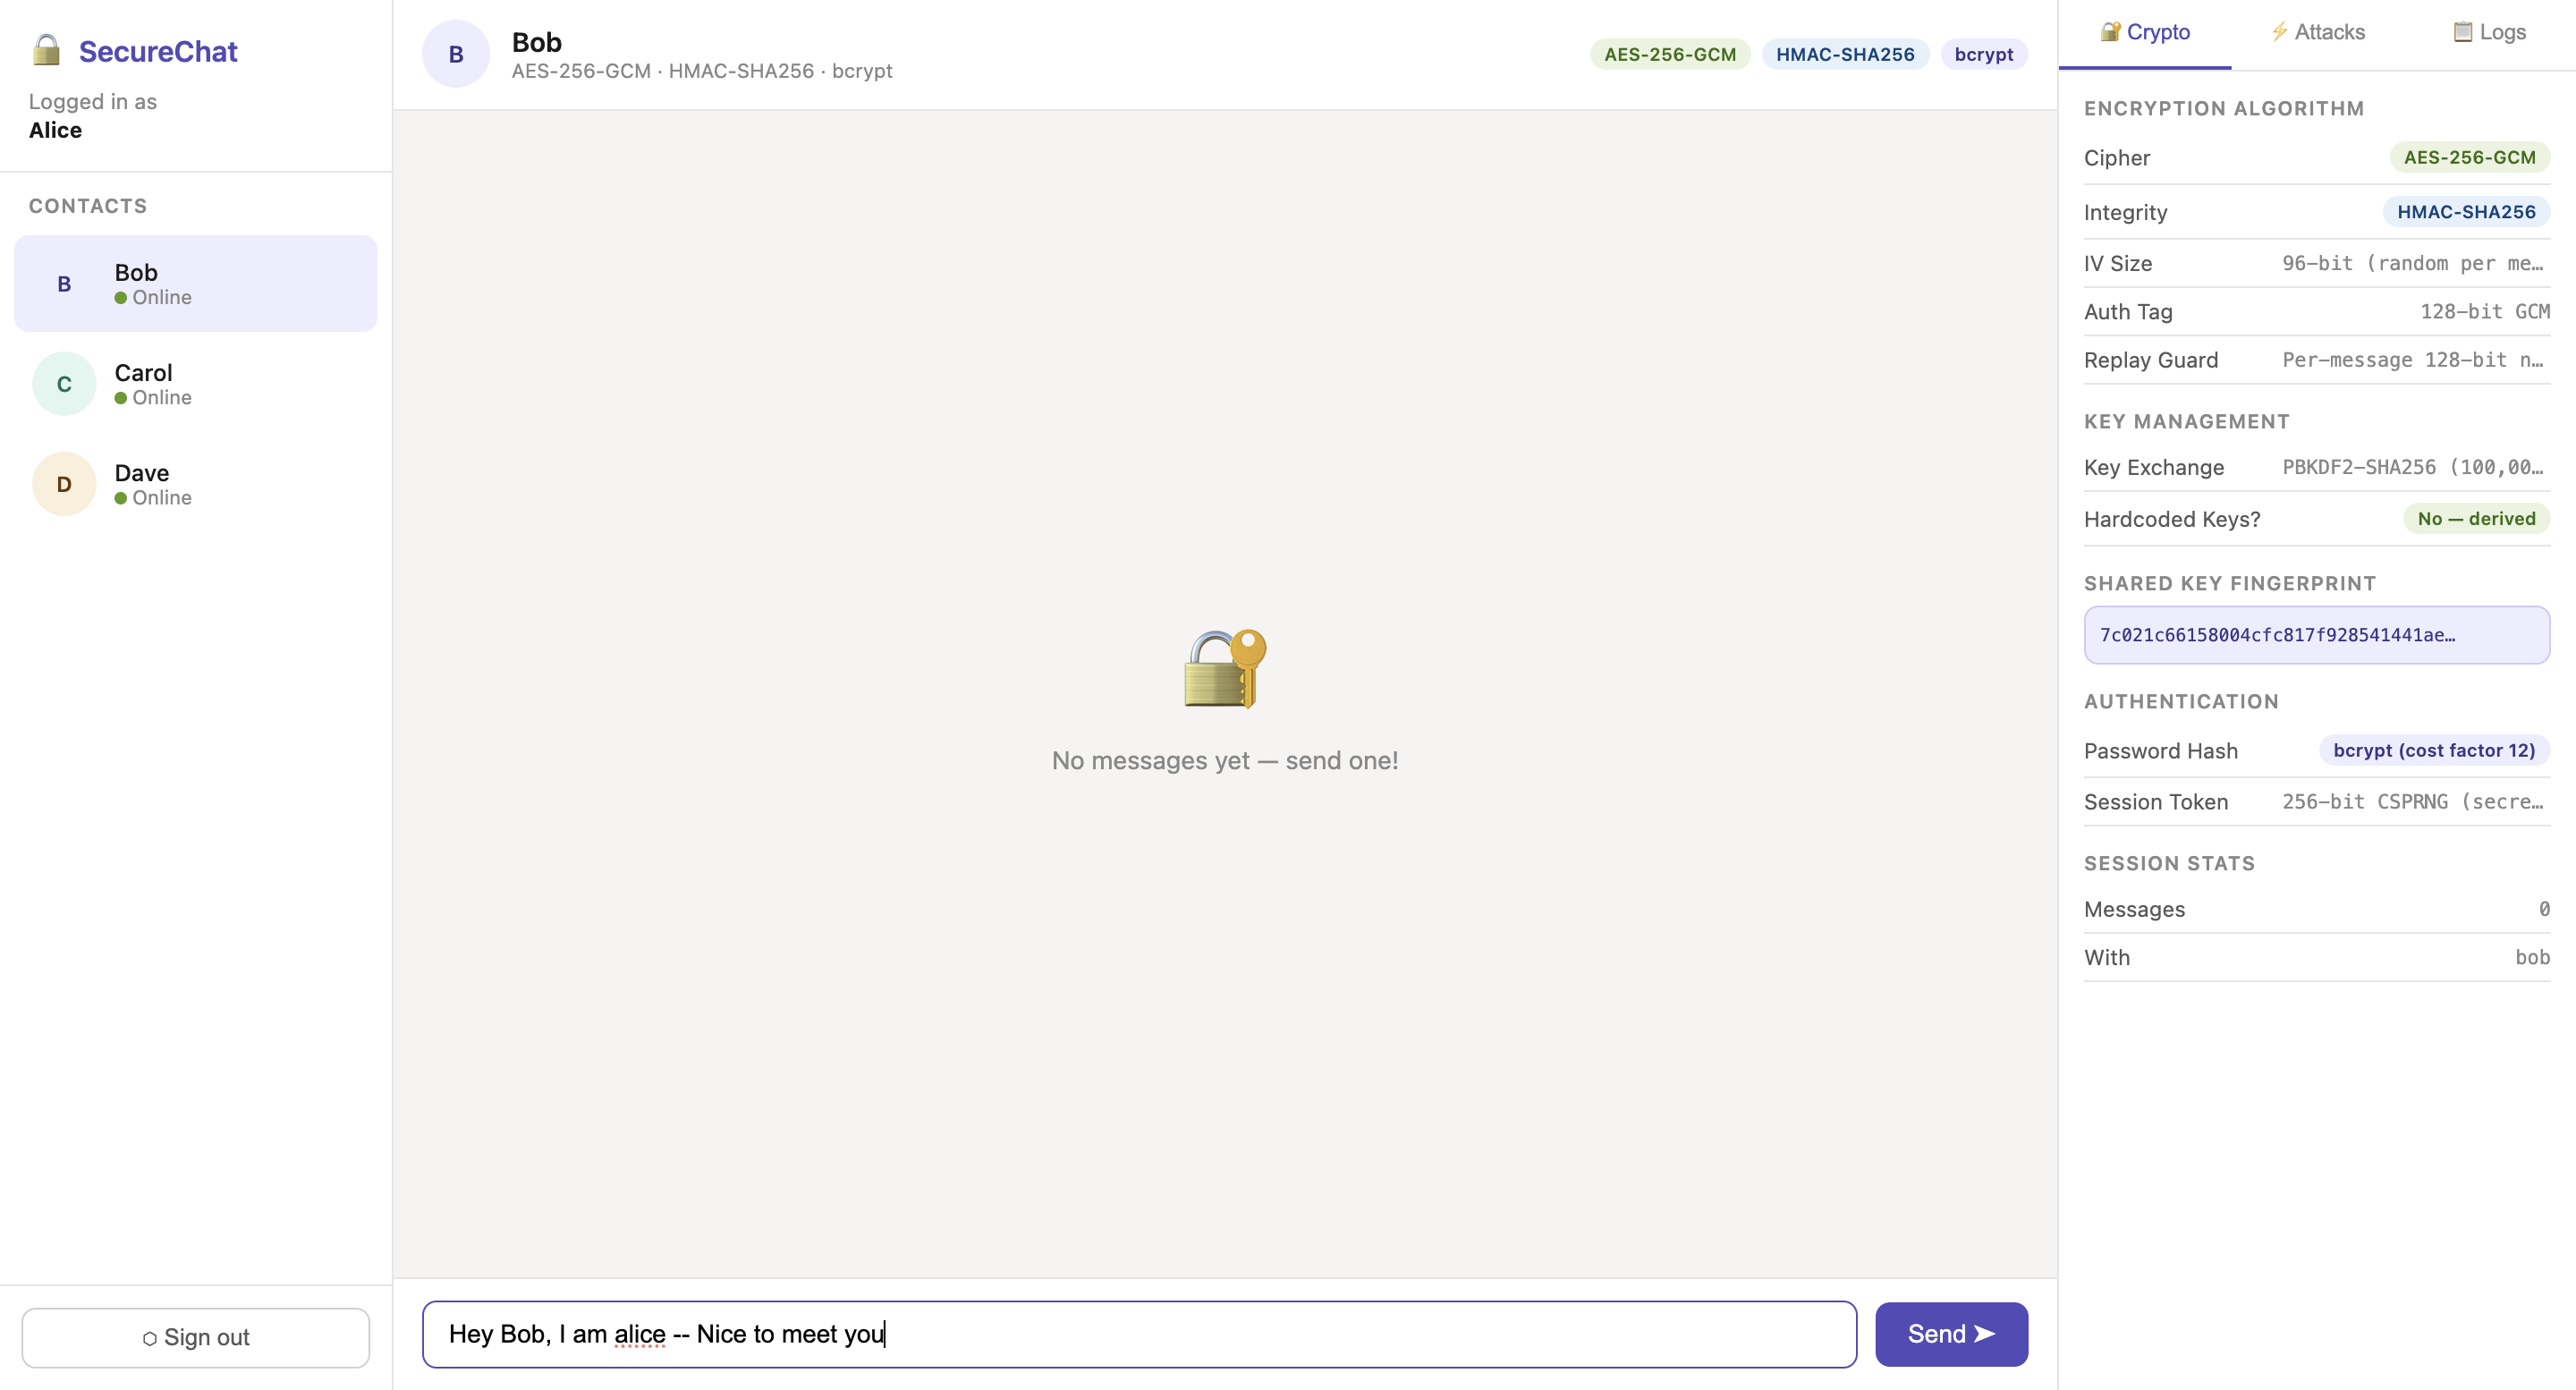
\includegraphics[width=\columnwidth]{sc_crypto_panel.png}
    \caption{The Crypto information panel reveals every parameter the system is using for the current conversation: the cipher, integrity algorithm, IV size, GCM auth tag length, key derivation function, the truncated shared-key fingerprint, the bcrypt cost factor, and the session-token entropy. No values are hardcoded --- all are computed at runtime.}
    \label{fig:crypto_panel}
\end{figure}

% ─── IV. User Authentication ──────────────────────────────────────────────────
\section{User Authentication Module}
\label{sec:auth}

\subsection{Registration}
A new user supplies a username, display name, and password. The server applies a small set of validation rules --- usernames must be at least three characters long, passwords at least six --- and then computes the bcrypt hash before storing anything. The plaintext password is held in memory only for the duration of the request and is overwritten when the handler returns.

\begin{lstlisting}[caption={Password hashing routine.}]
def hash_password(password: str) -> bytes:
    return bcrypt.hashpw(
        password.encode("utf-8"),
        bcrypt.gensalt(rounds=12)
    )
\end{lstlisting}

\subsection{Login and Session Tokens}
The login handler retrieves the stored bcrypt hash for the requested username and uses \texttt{bcrypt.checkpw} to verify the supplied password. On success, a session token is generated by \texttt{secrets.token\_hex(32)}, producing 32 random bytes (256 bits) encoded as 64 hexadecimal characters. The token is stored server-side in a dictionary indexed by the token itself, with the username, login timestamp, and originating IP address as the associated record.

\subsection{Account Lockout}
Five consecutive failed login attempts for a given username will lock the account. The lockout check runs \emph{before} password verification, so a locked account incurs no further bcrypt work --- this prevents an attacker from using the lockout window as a timing oracle. Figure~\ref{fig:login_fail} shows the system's response after a single failed attempt: the user is told how many tries remain before the account is sealed.

\begin{figure}[H]
    \centering
    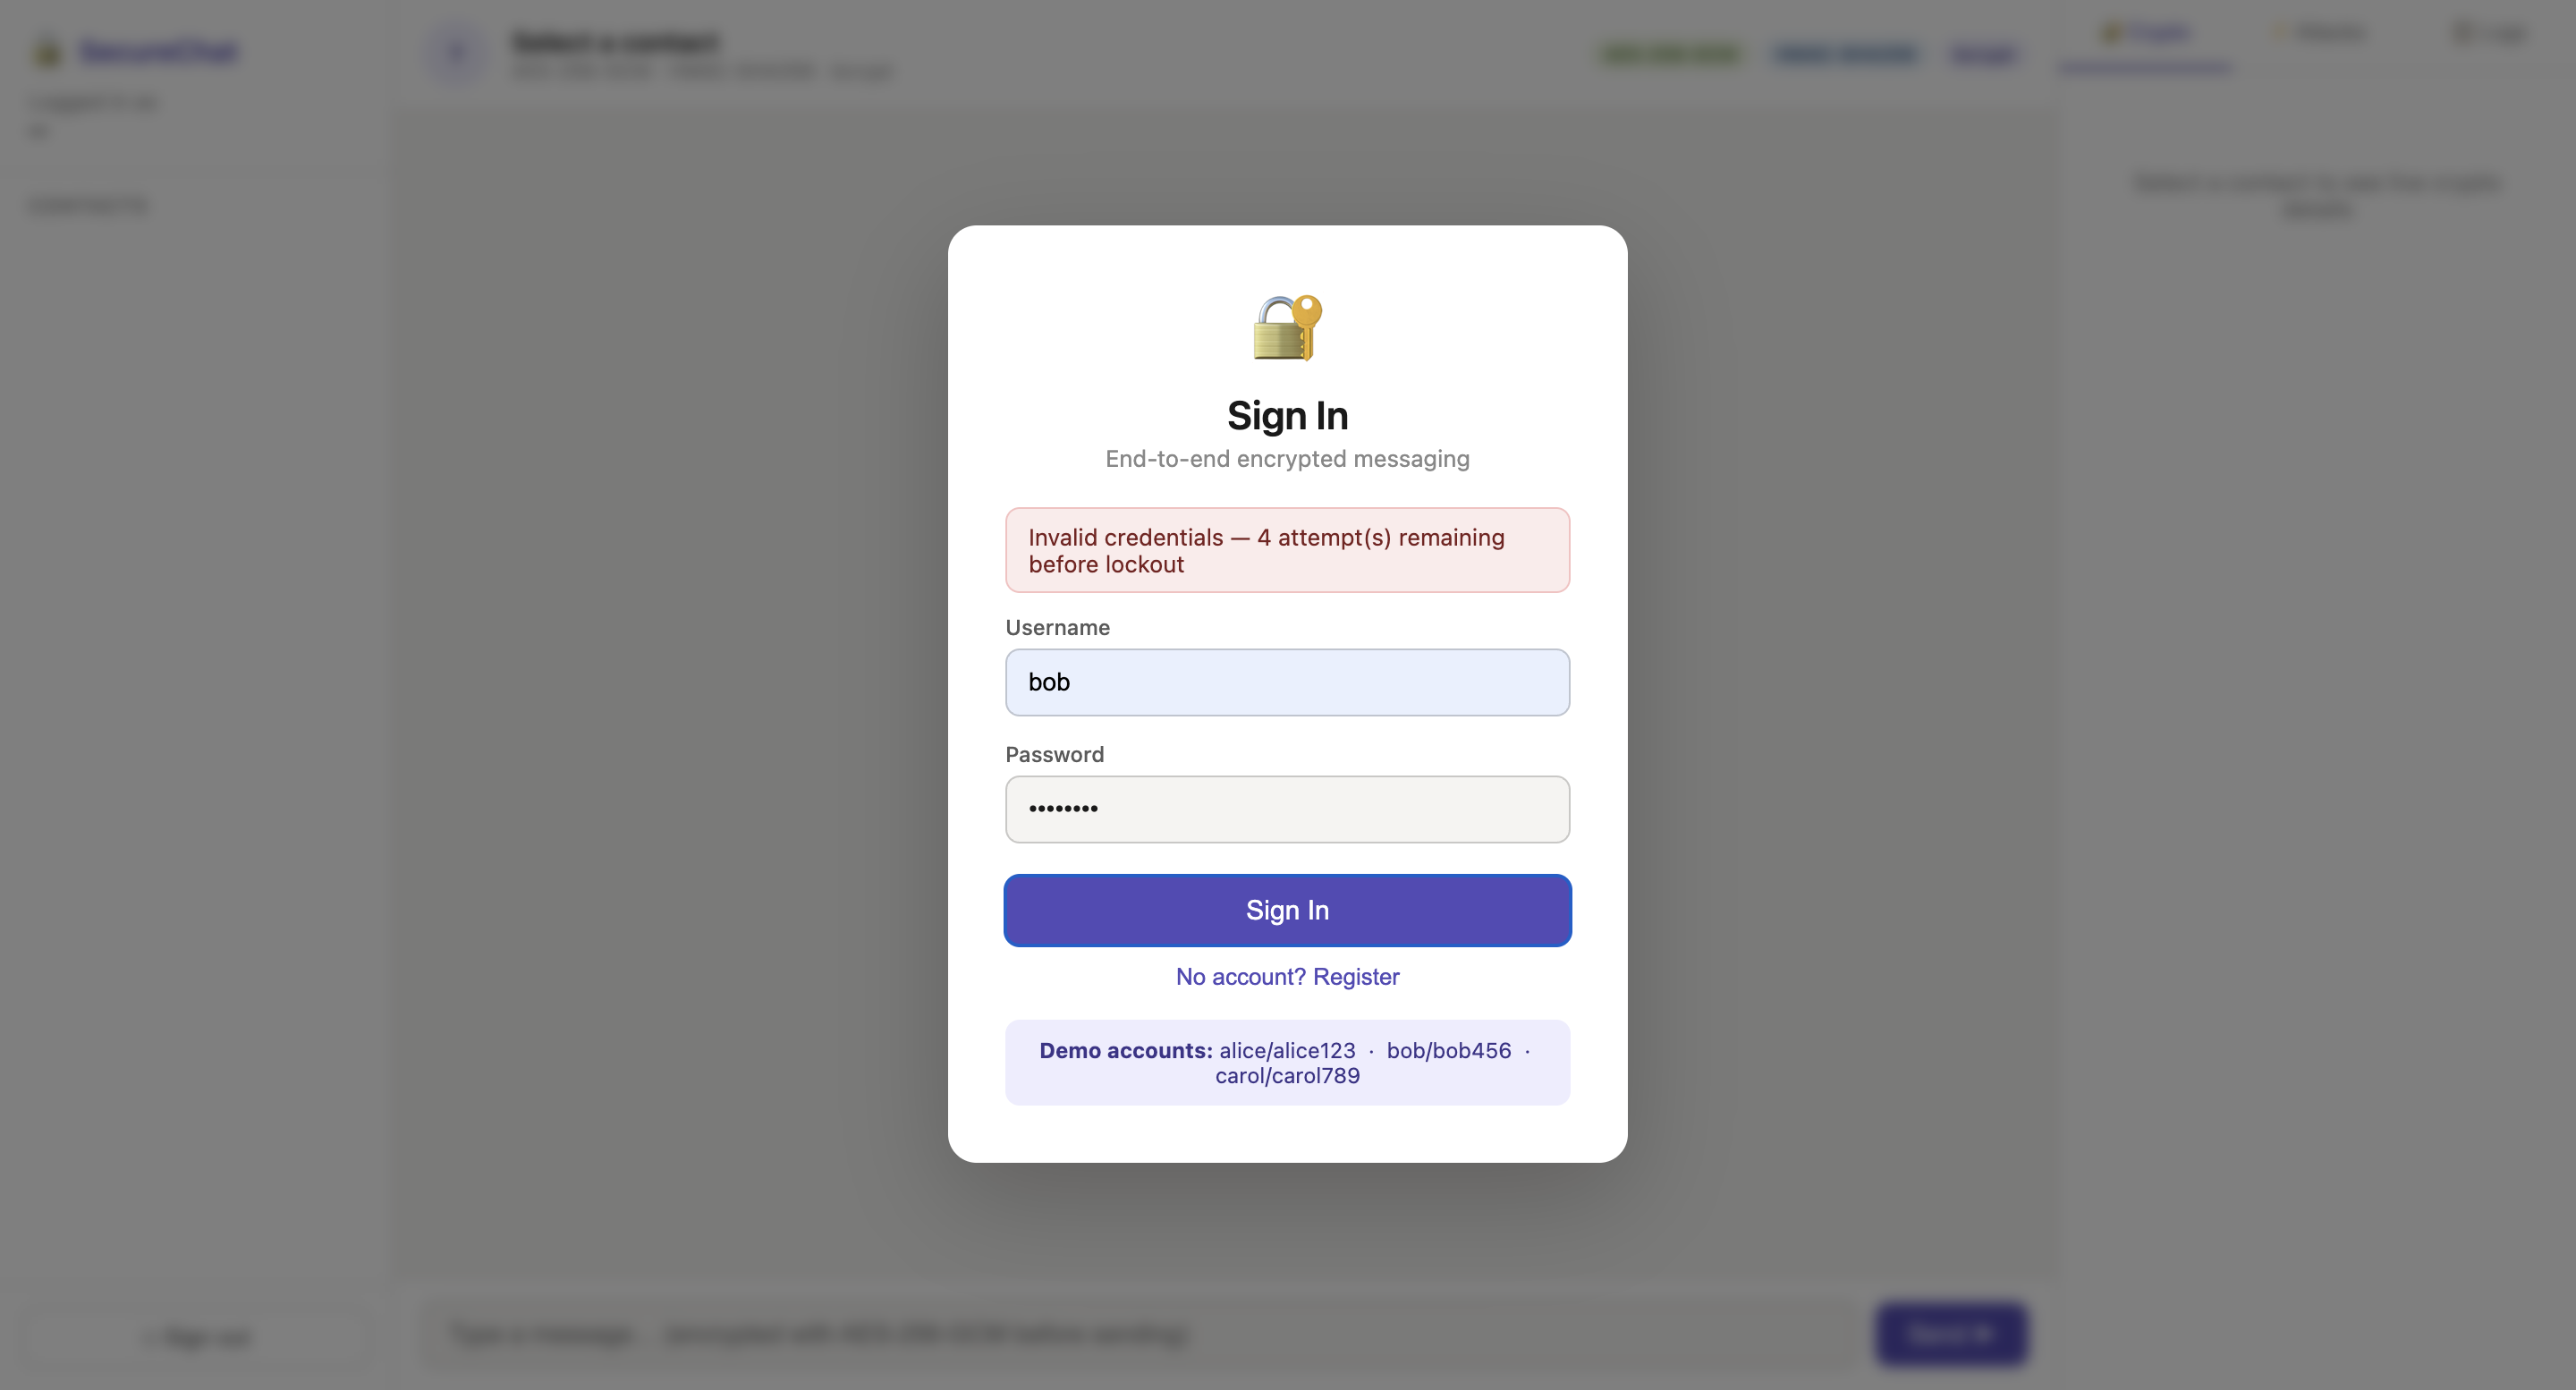
\includegraphics[width=\columnwidth]{sc_login_fail.png}
    \caption{Failed login attempt. The remaining count is displayed deliberately, both as a usability cue and as a clear signal that the system is enforcing a per-account limit.}
    \label{fig:login_fail}
\end{figure}

% ─── V. Symmetric Encryption ─────────────────────────────────────────────────
\section{Symmetric Encryption}
\label{sec:encryption}

\subsection{Why Key Derivation, Not Hardcoded Keys}
The single most important security property of any encryption system is that the key is not predictable. Embedding a key in source code violates this property in the worst possible way: anyone with read access to the repository immediately holds the key. SecureTalk avoids this by deriving every key at runtime.

For each pair of users $(A, B)$, an AES-256 key is generated by feeding the sorted pair of usernames, salted with the server's secret, into PBKDF2-SHA256:

\begin{lstlisting}[caption={Per-pair AES-256 key derivation.}]
def derive_shared_key(user_a: str, user_b: str) -> bytes:
    pair = "__".join(sorted([user_a, user_b]))
    return hashlib.pbkdf2_hmac(
        "sha256",
        pair.encode(),
        app.secret_key.encode(),
        iterations=100_000,
        dklen=32   # 256-bit output
    )
\end{lstlisting}

The sort ensures that \texttt{derive\_shared\_key("alice","bob")} and \texttt{derive\_shared\_key("bob","alice")} produce the same key, so both ends of a conversation arrive at the same value without coordination. The HMAC key for the same pair is derived independently using a different salt suffix, ensuring that the HMAC key and the encryption key are cryptographically unrelated.

\subsection{Per-Message Encryption}
Encrypting a single message takes a small, fixed sequence of operations:

\begin{lstlisting}[caption={AES-256-GCM encryption of one message.}]
iv         = os.urandom(12)        # 96-bit random IV
msg_nonce  = secrets.token_hex(16) # 128-bit unique nonce
nonce_store.add(msg_nonce)         # register immediately

aesgcm     = AESGCM(key)
ciphertext = aesgcm.encrypt(
    iv, plaintext.encode("utf-8"), None
)
\end{lstlisting}

The 96-bit IV is drawn freshly from the operating system's CSPRNG for every single message. With 96 random bits, the probability of an accidental IV collision under the same key is negligible for any realistic message volume.

\subsection{What the User Sees}
Figure~\ref{fig:msg_sent} shows the result of Alice sending the message ``Hey Bob, I am alice -- Nice to meet you'' to Bob. The bubble itself contains the plaintext (Alice can of course read what she just typed), but the line below it reveals the ciphertext preview that was actually stored and transmitted: \texttt{NWTj9UbK2Xpx0QXUr6duqxAVQmqnv3Wu\dots}. The small \texttt{HMAC} and \texttt{AES-256-GCM} badges confirm that both integrity and encryption are in effect for this particular message.

\begin{figure}[H]
    \centering
    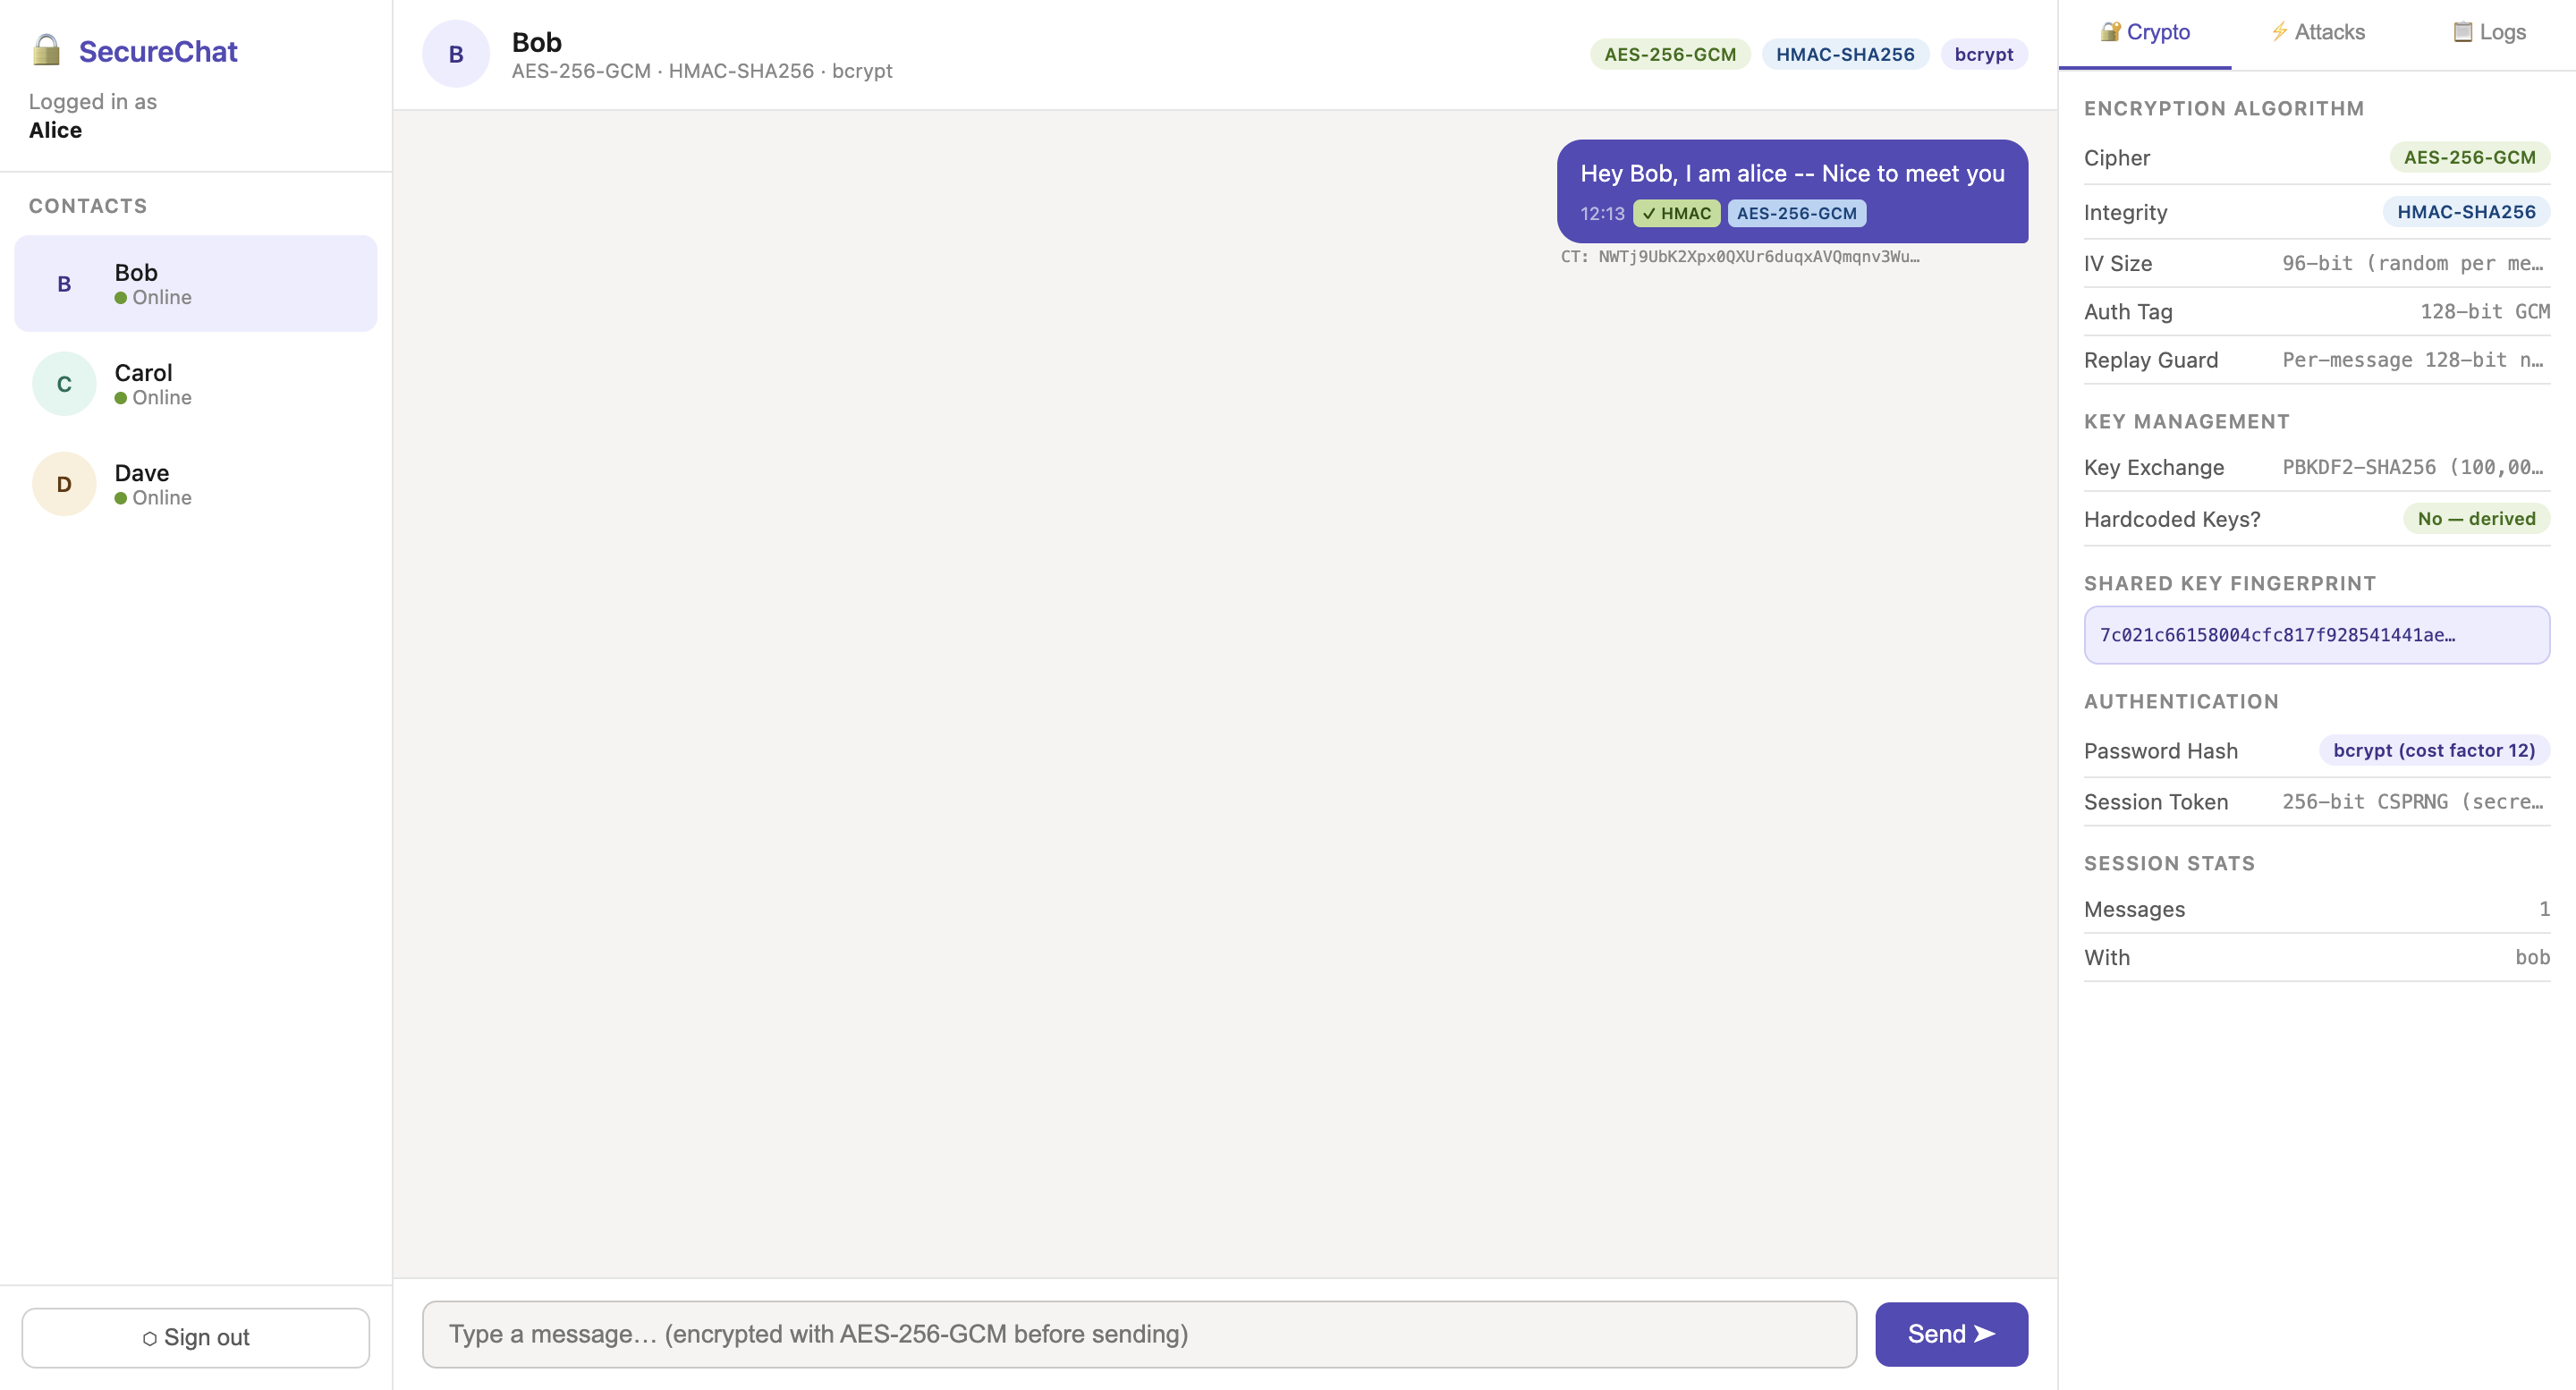
\includegraphics[width=\columnwidth]{sc_message_sent.png}
    \caption{Alice's view immediately after sending a message. The ciphertext preview directly below the bubble is the only form in which the message actually exists in the server's storage.}
    \label{fig:msg_sent}
\end{figure}

Figure~\ref{fig:msg_received} shows the same message arriving at Bob's session, delivered in real time over SocketIO. The ciphertext shown to Bob is byte-for-byte identical to what Alice saw, but the decrypted plaintext only appears after the HMAC has been verified and AES-GCM has confirmed the auth tag.

\begin{figure}[H]
    \centering
    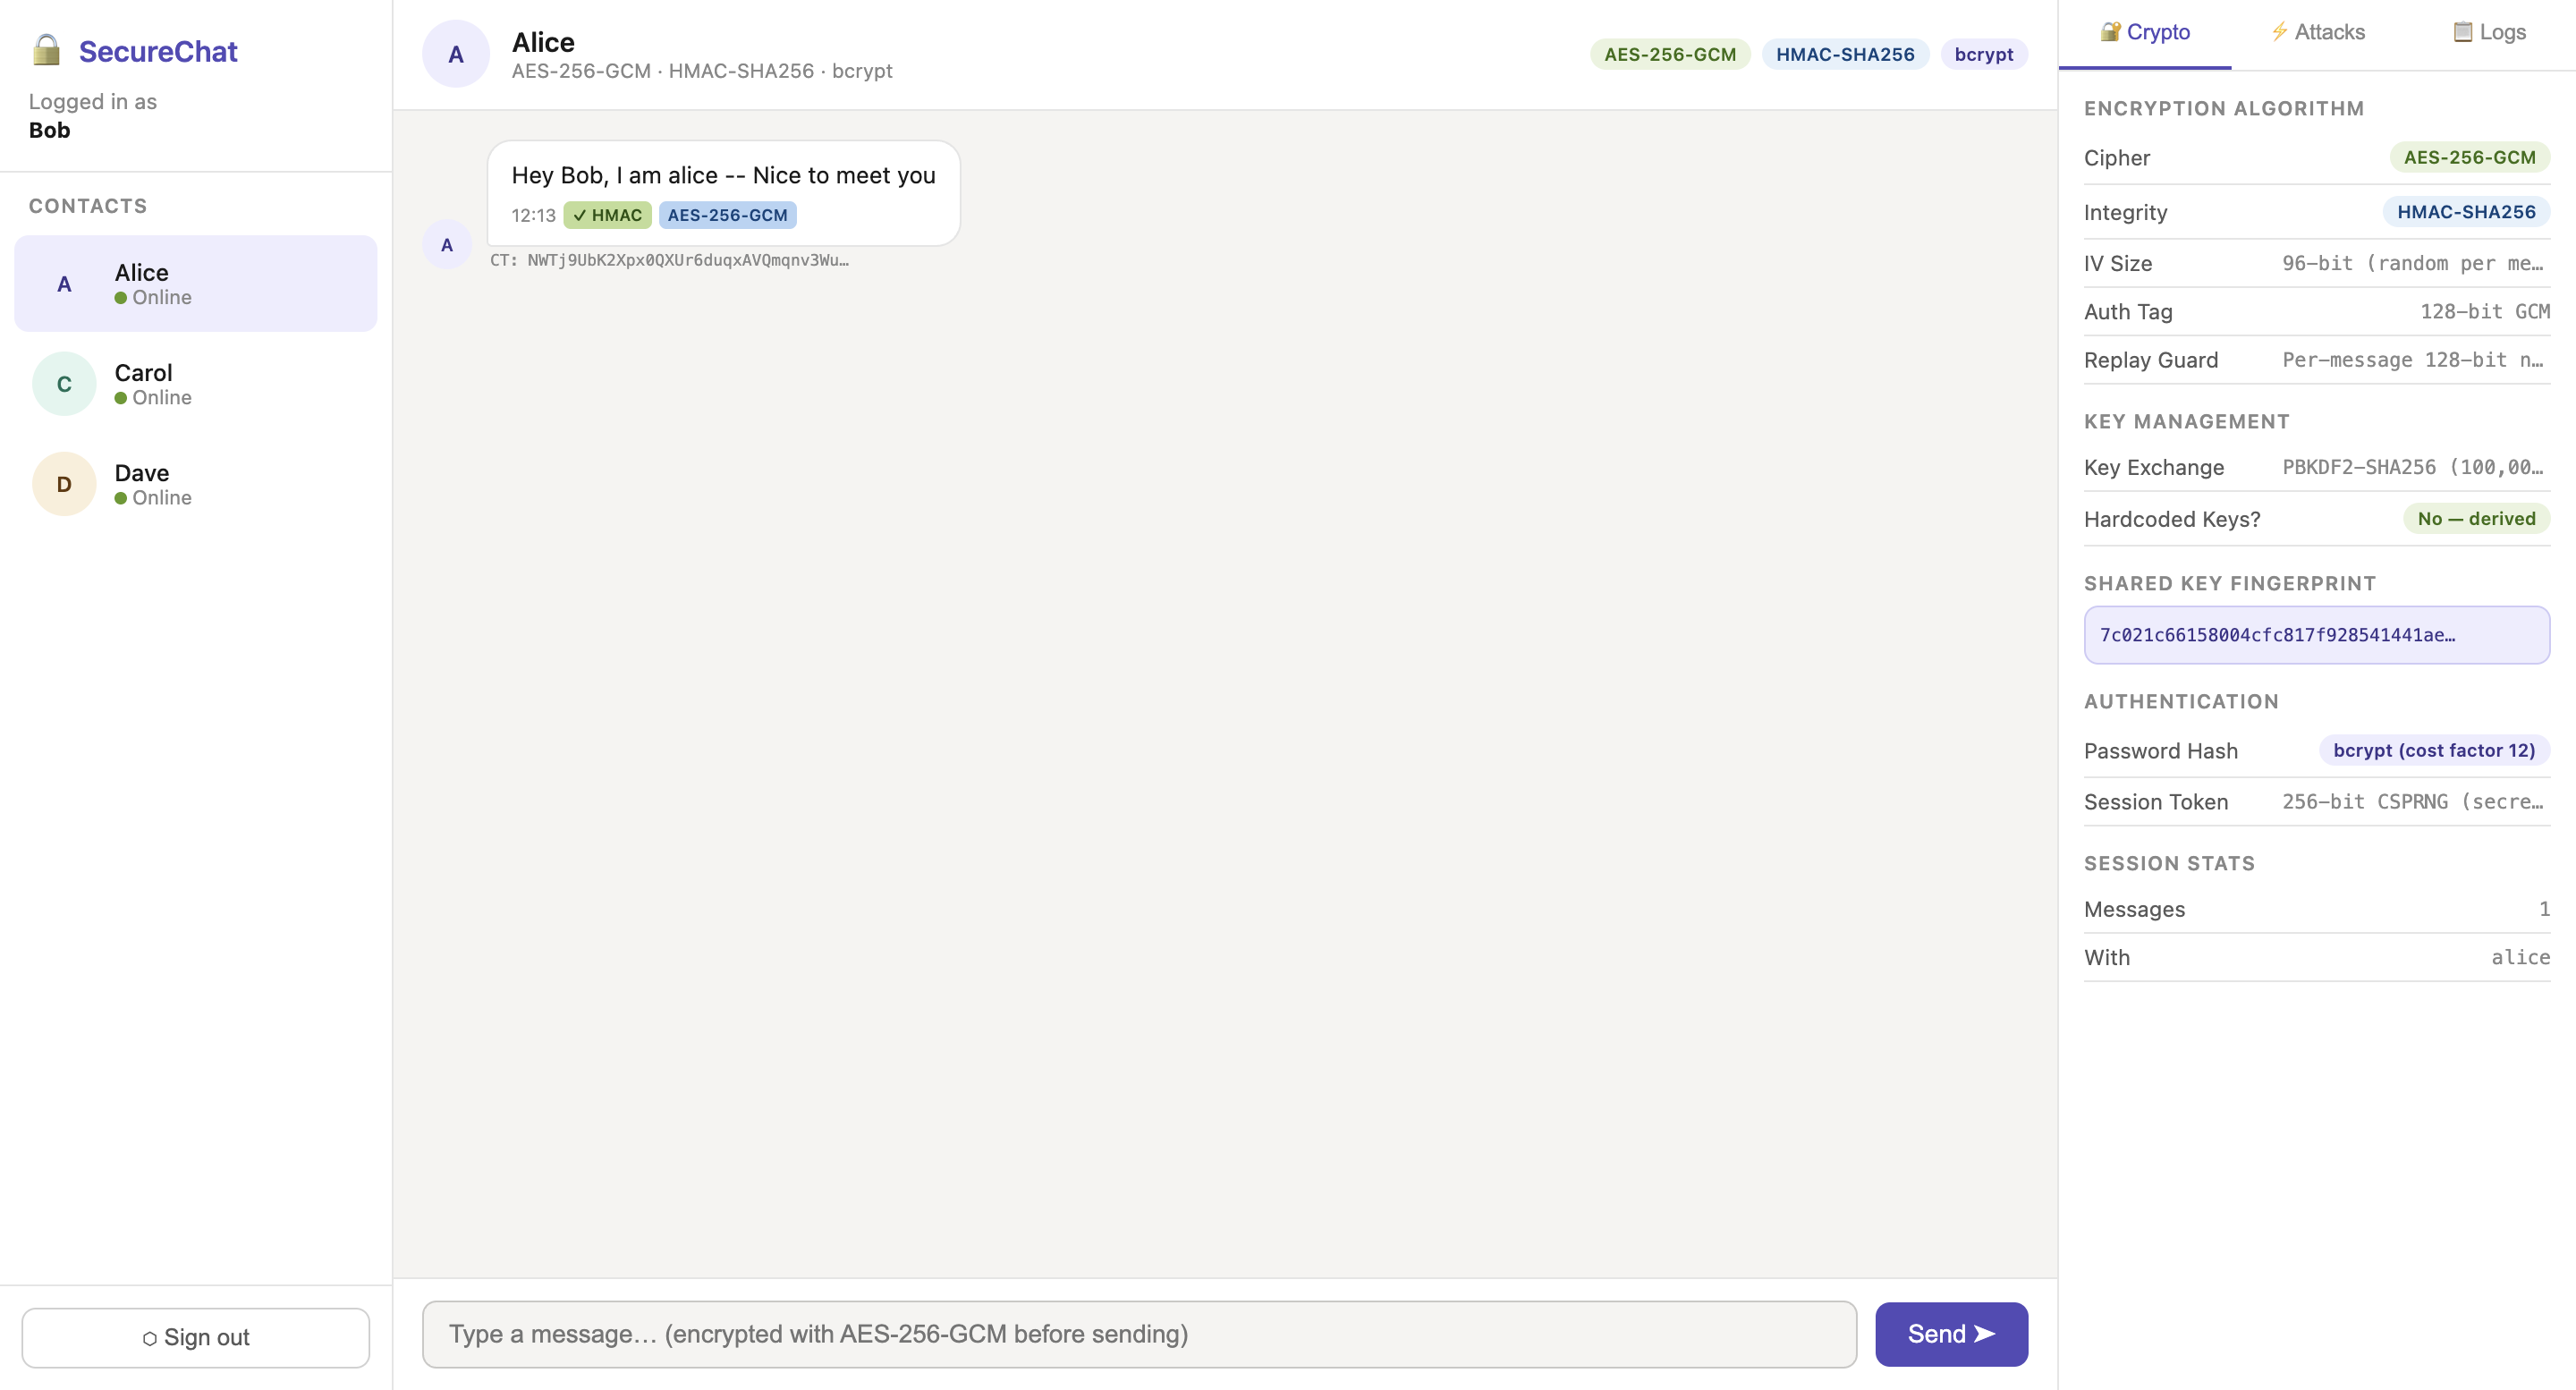
\includegraphics[width=\columnwidth]{sc_message_received.png}
    \caption{Bob's view of the same message after real-time delivery. The system verifies the HMAC, then decrypts, and only then renders the plaintext.}
    \label{fig:msg_received}
\end{figure}

% ─── VI. Message Integrity ────────────────────────────────────────────────────
\section{Message Integrity}
\label{sec:integrity}

\subsection{The HMAC Layer}
After encryption, an HMAC-SHA256 is computed over the raw ciphertext bytes:

\begin{lstlisting}[caption={HMAC computation over the ciphertext.}]
h   = hmac.new(hmac_key, ciphertext, hashlib.sha256)
mac = h.hexdigest()
\end{lstlisting}

This tag is stored alongside the ciphertext, the IV, and the nonce. When the message is later read, the recipient recomputes the HMAC and compares the result using \texttt{hmac.compare\_digest}. The use of constant-time comparison is deliberate --- a naive \texttt{==} comparison would leak information about the position of any mismatching byte through its timing behaviour, which over many trials can be exploited by an attacker to forge a valid tag \cite{kocher1996timing}.

\begin{lstlisting}[caption={Constant-time HMAC verification.}]
expected = hmac.new(hmac_key, ciphertext, hashlib.sha256)
expected_mac = expected.hexdigest()
if not hmac.compare_digest(expected_mac, enc["hmac"]):
    raise ValueError(
        "HMAC verification failed -- "
        "message integrity compromised"
    )
\end{lstlisting}

\subsection{Why Two Integrity Layers}
A reasonable question is why HMAC is used at all, given that AES-GCM already provides authenticated encryption. The answer is defence in depth. If a future bug in the encryption code path were to skip the auth-tag check (this has happened in real systems), the separate HMAC layer would still catch tampered ciphertext before the decryption code is even called. In addition, the HMAC tag is exposed in the message metadata, which makes the integrity check visually inspectable in the interface --- a property that is useful both as a learning aid and as a real audit feature.

% ─── VII. Attack Simulations ──────────────────────────────────────────────────
\section{Attack Simulations}
\label{sec:attacks}

Three attacks were simulated, each accessible from the Attacks tab in the running application.

\subsection{Man-in-the-Middle: Tampering with the Ciphertext}
The first attack assumes an adversary positioned between Alice and the server, with the ability to read and modify the encrypted packet in flight. The simulation makes a deep copy of the most recent message --- never touching the original record stored in the server --- and flips three bytes in the copied ciphertext at positions 0, 5, and 10. The corrupted packet is then handed to the decryption pipeline.

\begin{figure}[H]
    \centering
    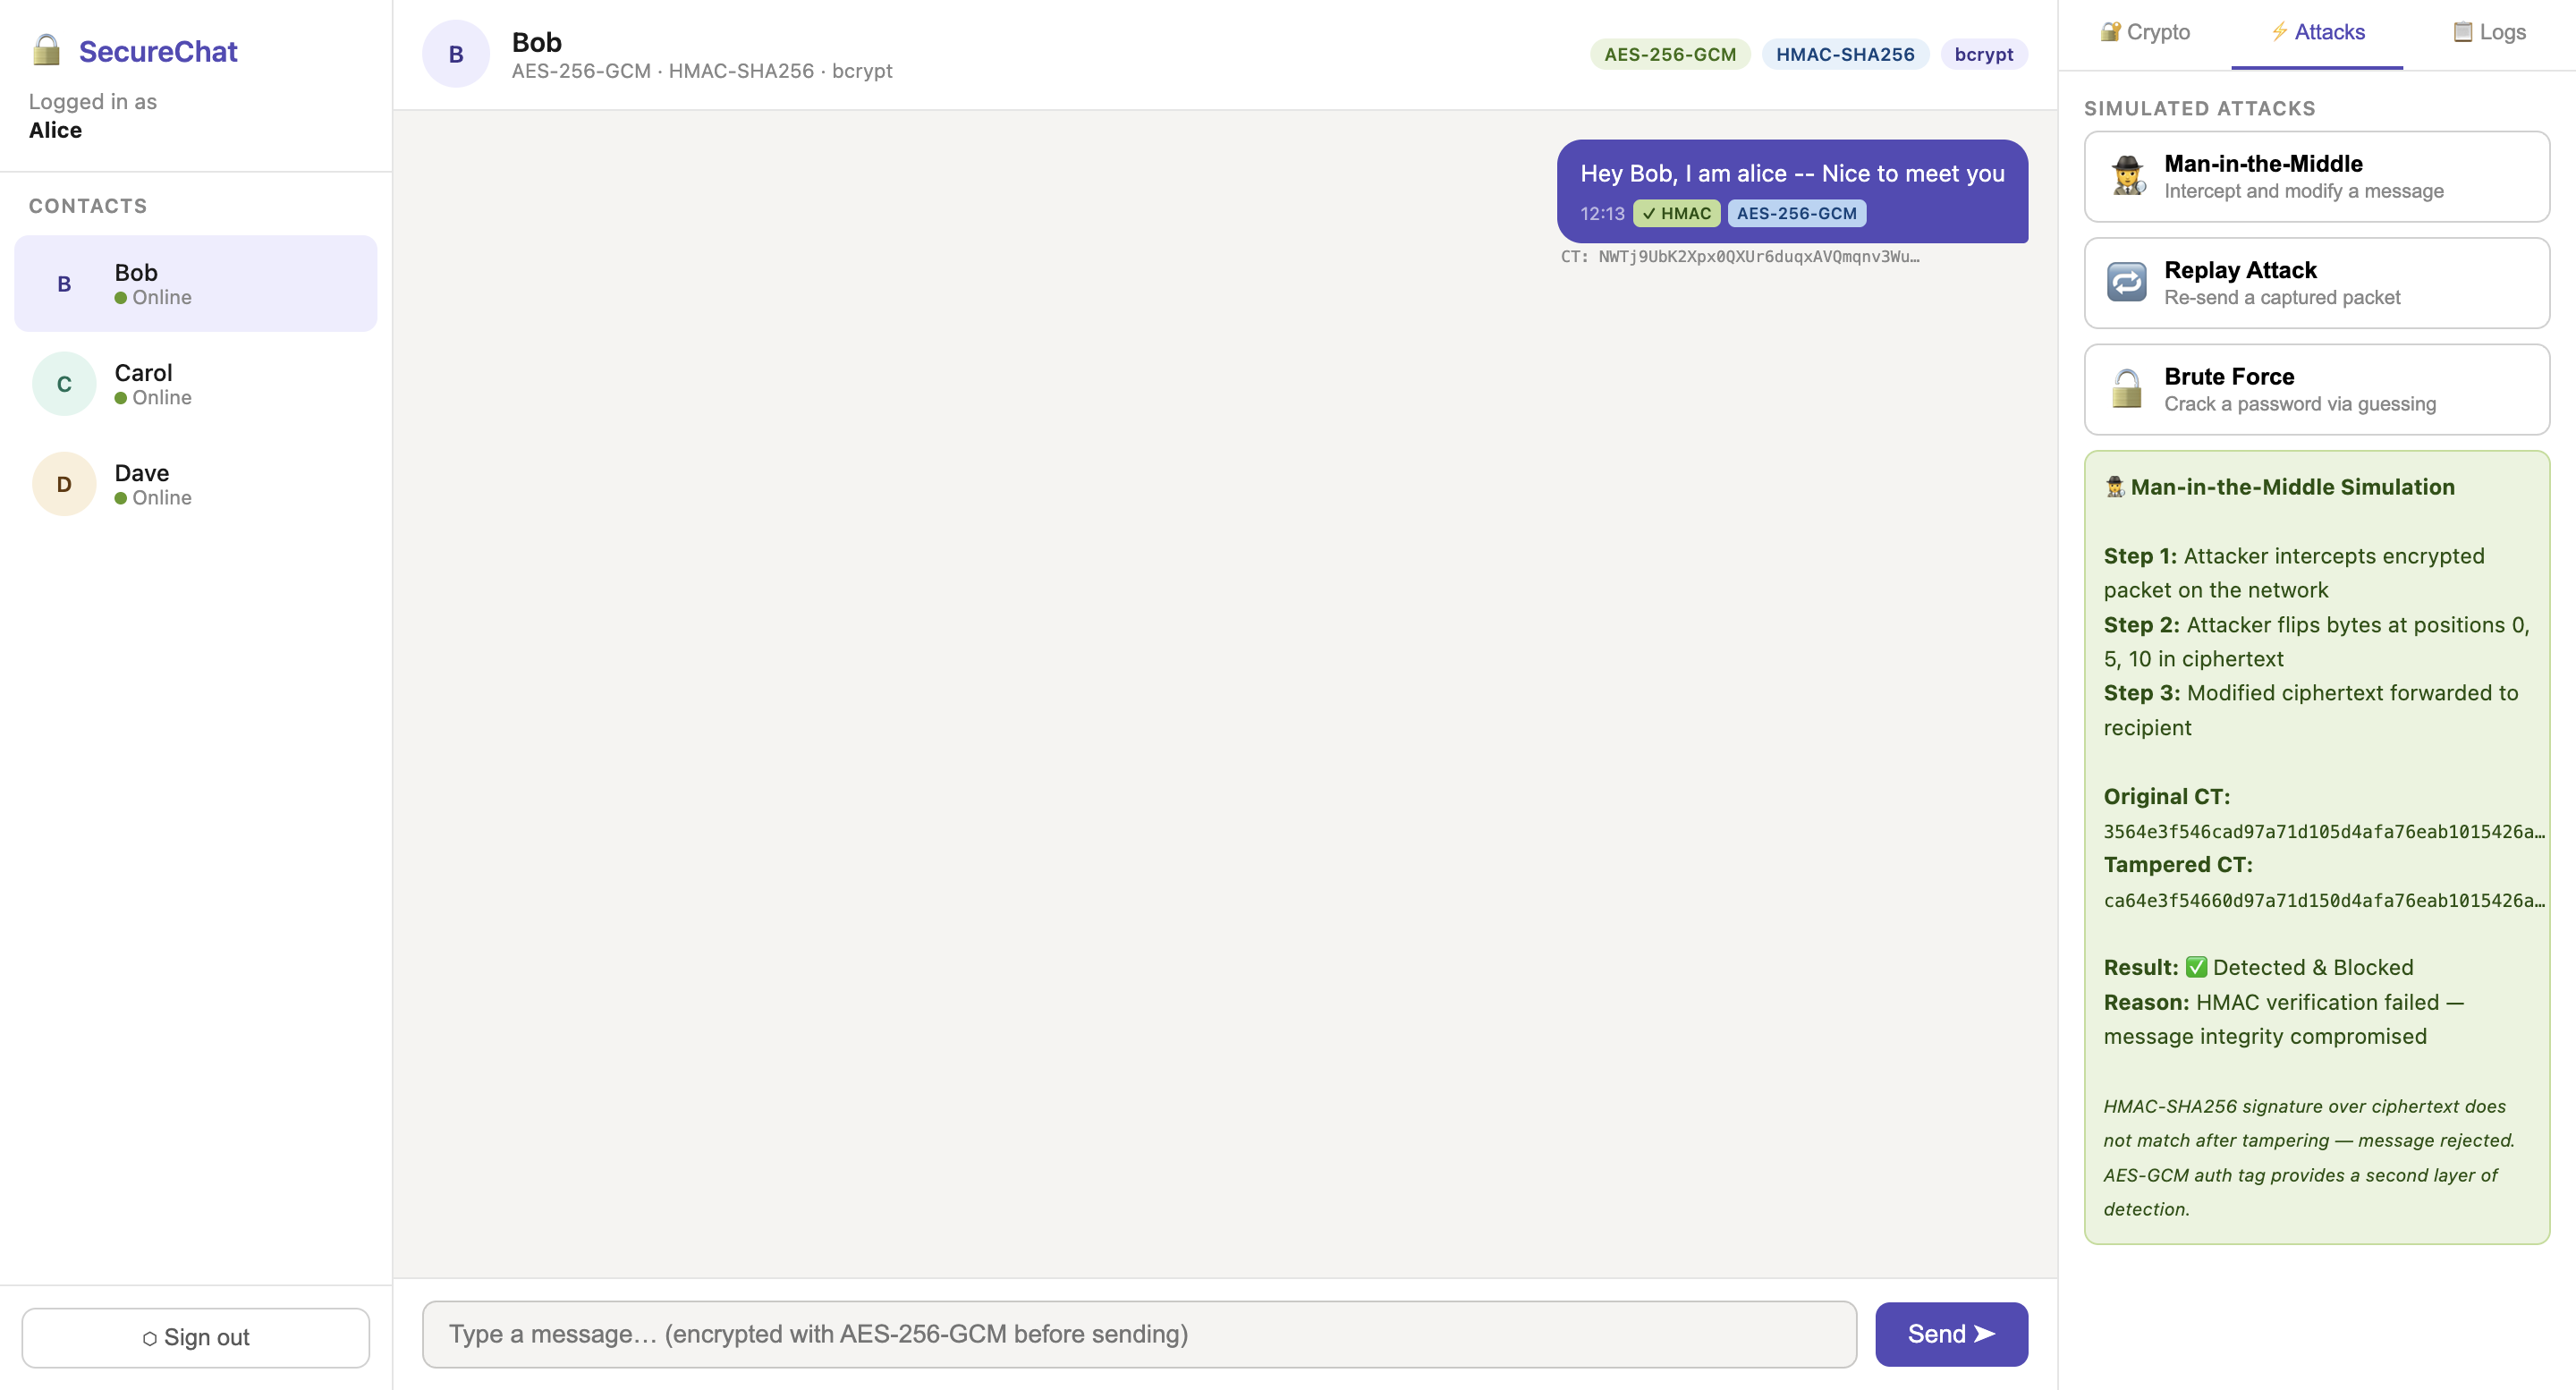
\includegraphics[width=\columnwidth]{sc_attack_mitm.png}
    \caption{MITM simulation. The original and tampered ciphertexts are displayed side-by-side; differences are easily spotted at the flipped positions. The HMAC verification step refuses the modified packet immediately, before any decryption is attempted.}
    \label{fig:mitm}
\end{figure}

As Figure~\ref{fig:mitm} shows, the tampering is caught immediately. The HMAC over the modified ciphertext no longer matches the stored tag, the verification function raises a \texttt{ValueError}, and the result panel reports ``\textbf{Detected \& Blocked}''. Even if the HMAC layer were somehow bypassed, the AES-GCM authentication tag would refuse to decrypt the modified ciphertext during the next stage --- two independent layers of protection both stop the same attack.

\subsection{Replay Attack: Re-Sending a Captured Packet}
The replay simulation assumes an adversary who managed to record a valid encrypted packet on the wire and now plays the same packet back to the server, hoping it will be accepted as fresh. Because the nonce of every legitimate message is added to a server-side set at the moment of sending, the replayed nonce is already present in the set when the duplicate arrives.

\begin{figure}[H]
    \centering
    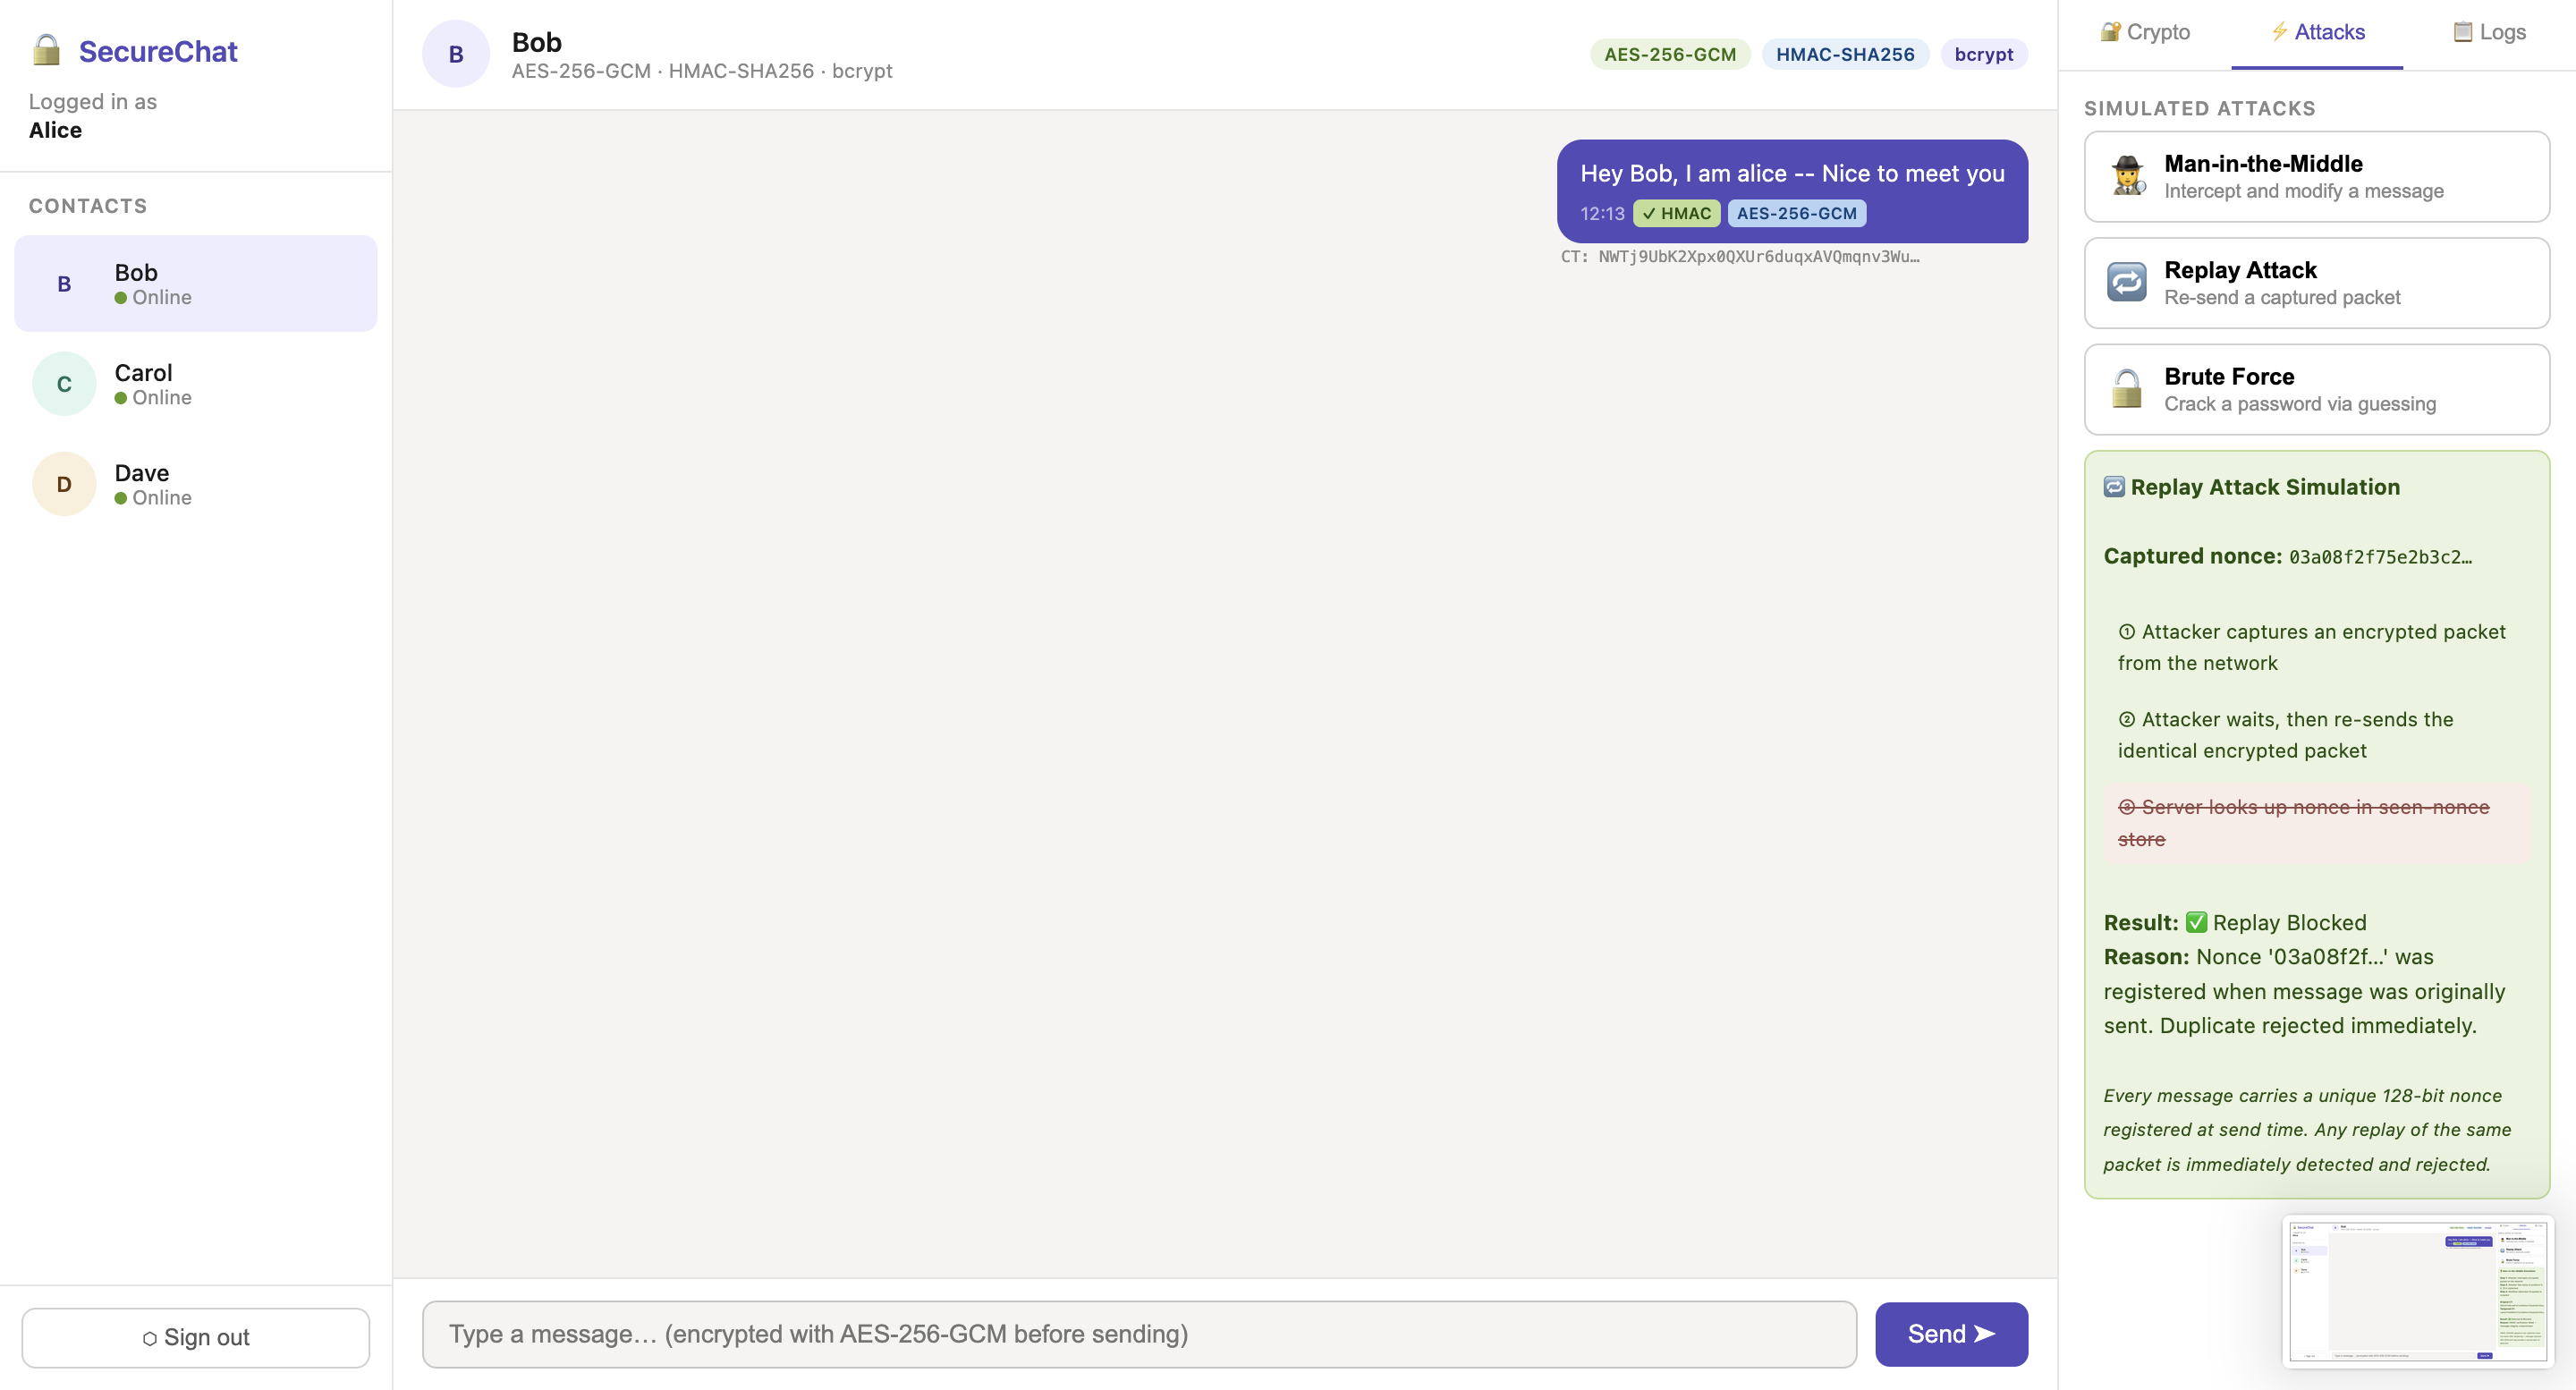
\includegraphics[width=\columnwidth]{sc_attack_replay.png}
    \caption{Replay attack simulation. The captured nonce \texttt{03a08f2f75e2b3c2\dots} is found in the server's seen-nonce store, and the duplicate is rejected without any cryptographic work being done.}
    \label{fig:replay}
\end{figure}

The detection in Figure~\ref{fig:replay} is essentially free in computational terms --- the system performs a single set membership test, not a full cryptographic verification. The result panel labels the duplicate ``Replay Blocked'' and identifies the offending nonce by its first eight hex characters.

\subsection{Brute Force: Guessing Passwords Offline}
The third simulation walks through a small dictionary of common passwords --- \textit{password}, \textit{123456}, \textit{letmein}, \textit{qwerty}, \textit{alice}, and so on --- and attempts each one against Alice's stored bcrypt hash. The point of the simulation is not to break the password (none of the guesses match) but to quantify how slow bcrypt makes each attempt.

\begin{figure}[H]
    \centering
    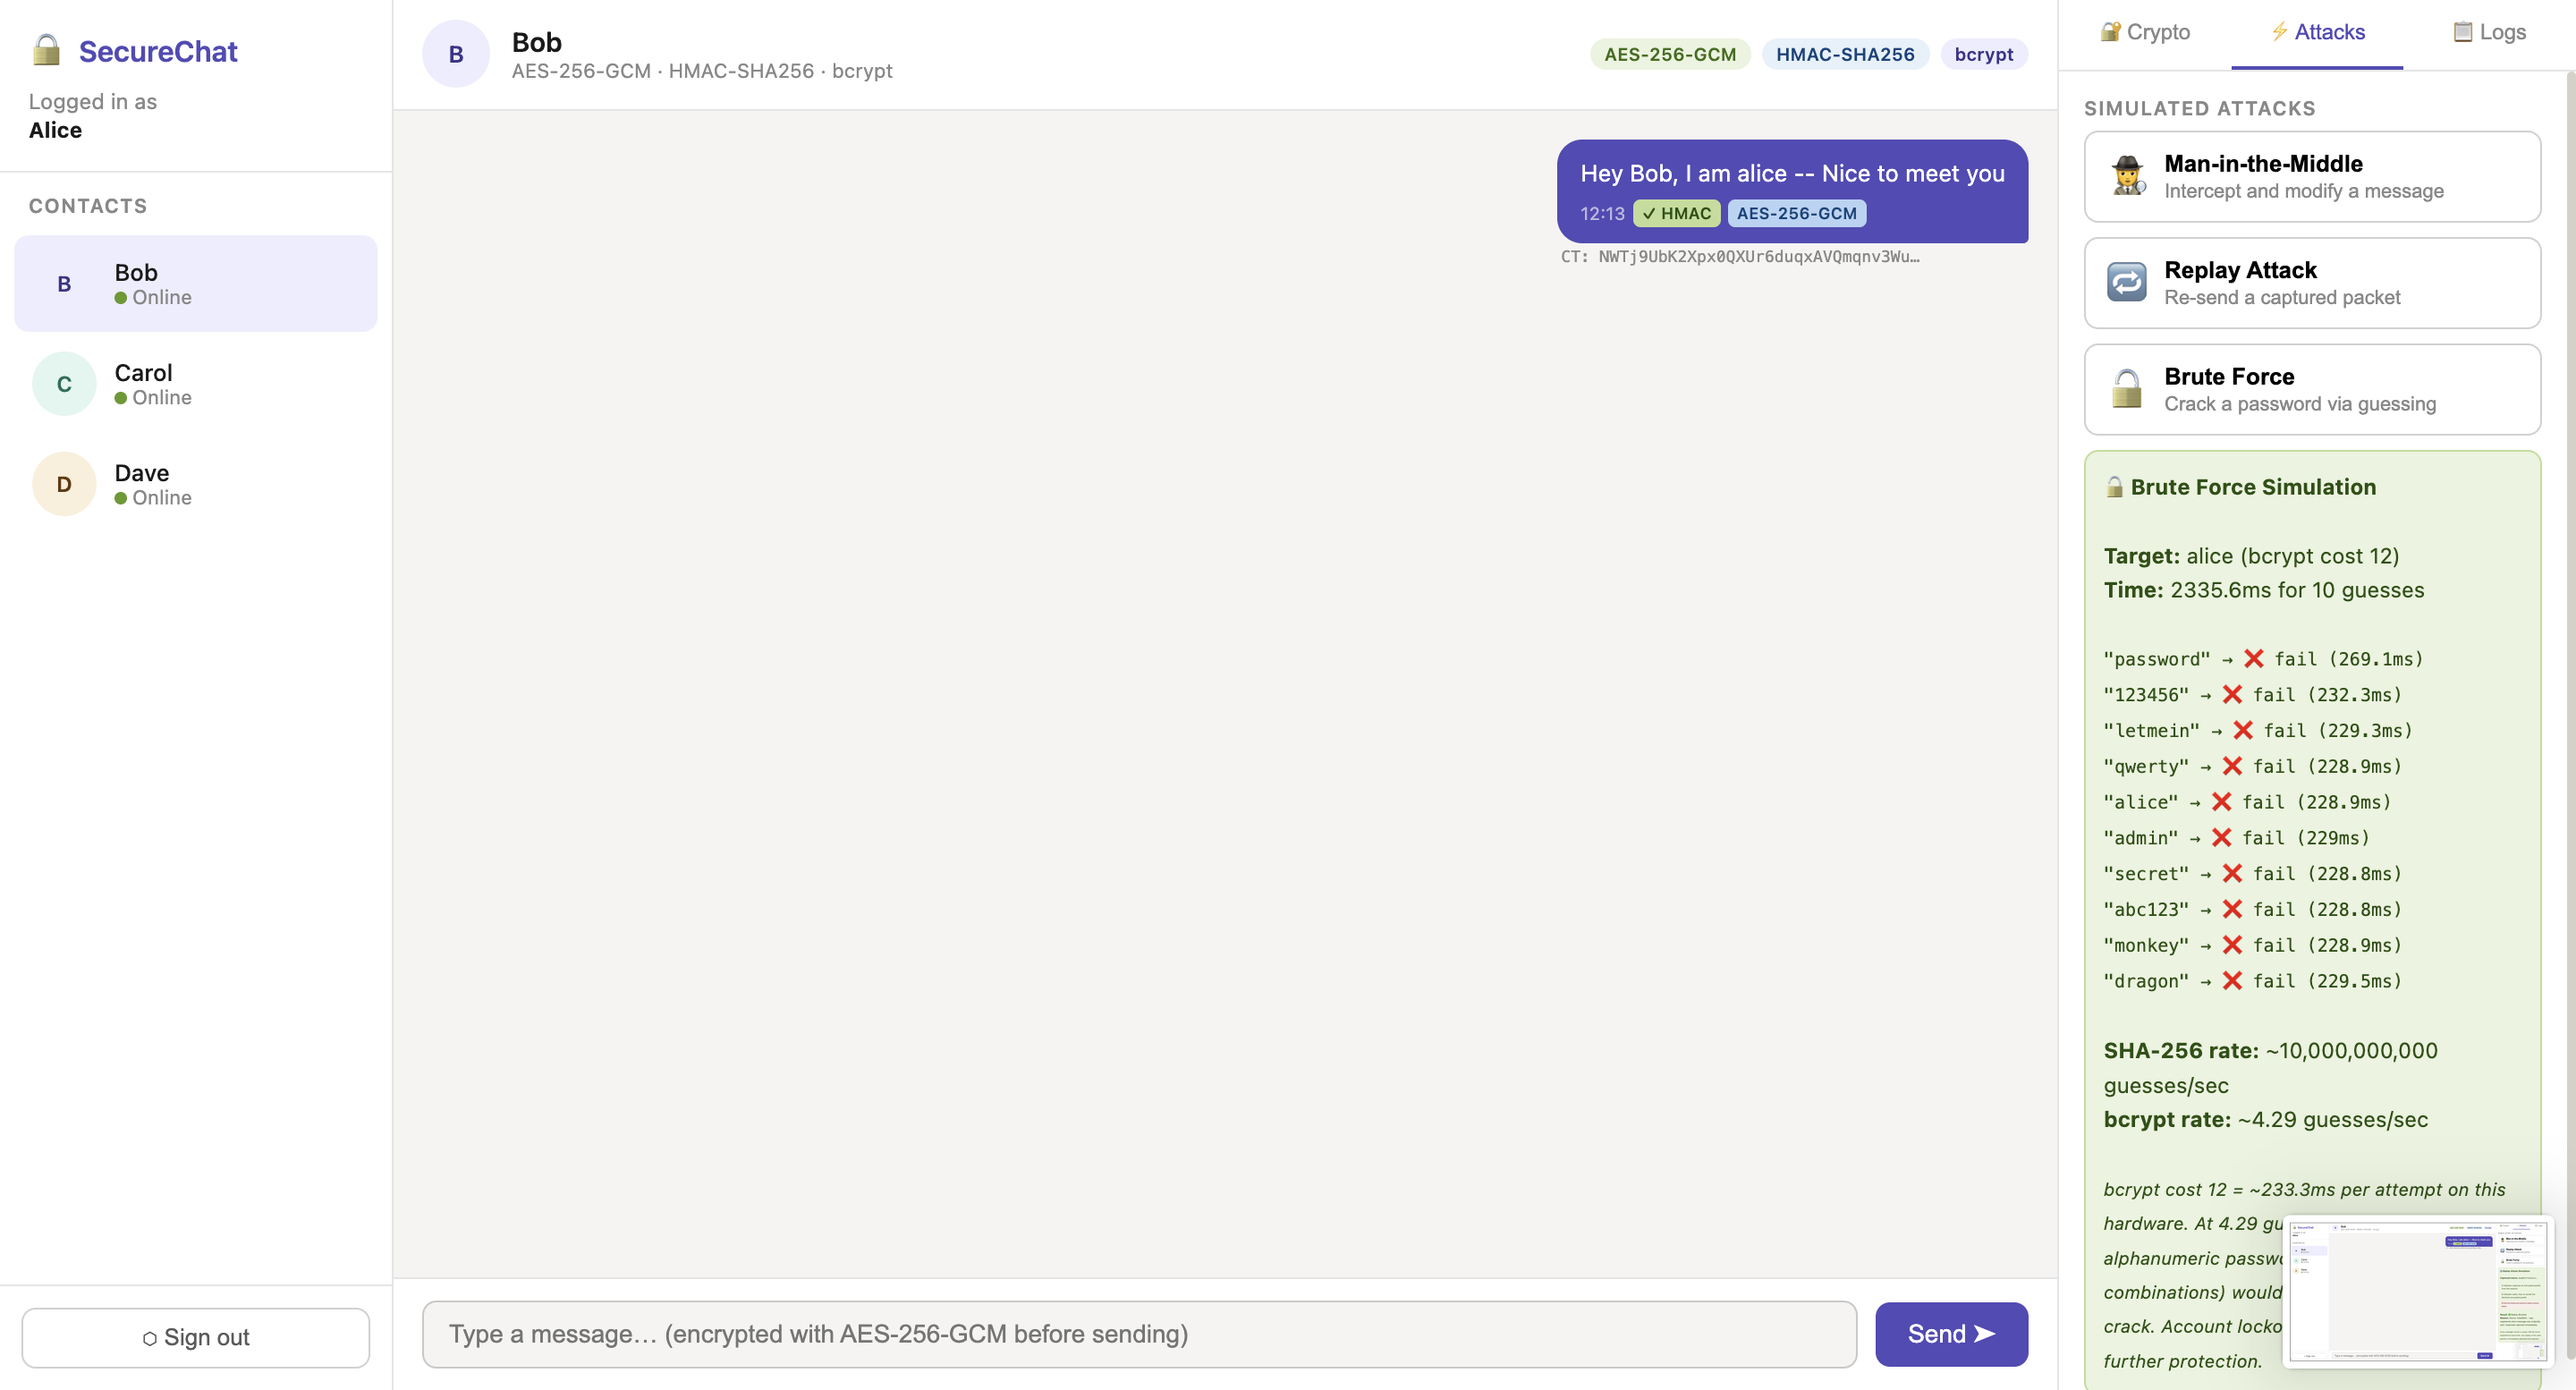
\includegraphics[width=\columnwidth]{sc_attack_bruteforce.png}
    \caption{Brute-force simulation. Each guess takes approximately 229\,ms on the test hardware. At this rate, the system supports only about 4.3 guesses per second --- many orders of magnitude slower than the billions per second possible against a raw SHA-256 hash.}
    \label{fig:brute}
\end{figure}

Figure~\ref{fig:brute} reports the measured timings. Each bcrypt verification takes between 228 and 269 milliseconds on the test hardware, yielding an effective rate of roughly 4.29 guesses per second. For comparison, an unsalted SHA-256 hash can be tested at approximately ten billion guesses per second on a modern GPU, so bcrypt is slowing the attacker by a factor on the order of $2 \times 10^9$. An eight-character lower-case-plus-digits password has $36^8 \approx 2.8 \times 10^{12}$ possible values, which at 4.29 guesses per second would take on the order of $20{,}000$ years to exhaust. In addition, the real login endpoint locks the account after five failures, which removes online guessing as an option entirely.

% ─── VIII. Logging System ─────────────────────────────────────────────────────
\section{Logging System}
\label{sec:logging}

Every security-relevant event is recorded with a timestamp, a level (INFO, WARNING, or ERROR), an event-type code, a human-readable message, and the associated username. Events are emitted simultaneously to the standard logging system (which writes \texttt{logs/security.log}) and to an in-memory ring buffer of the most recent two hundred entries. The frontend polls the buffer through the \texttt{/api/logs} endpoint and renders it in the Logs tab in real time, as shown in Figure~\ref{fig:logs}.

\begin{figure}[H]
    \centering
    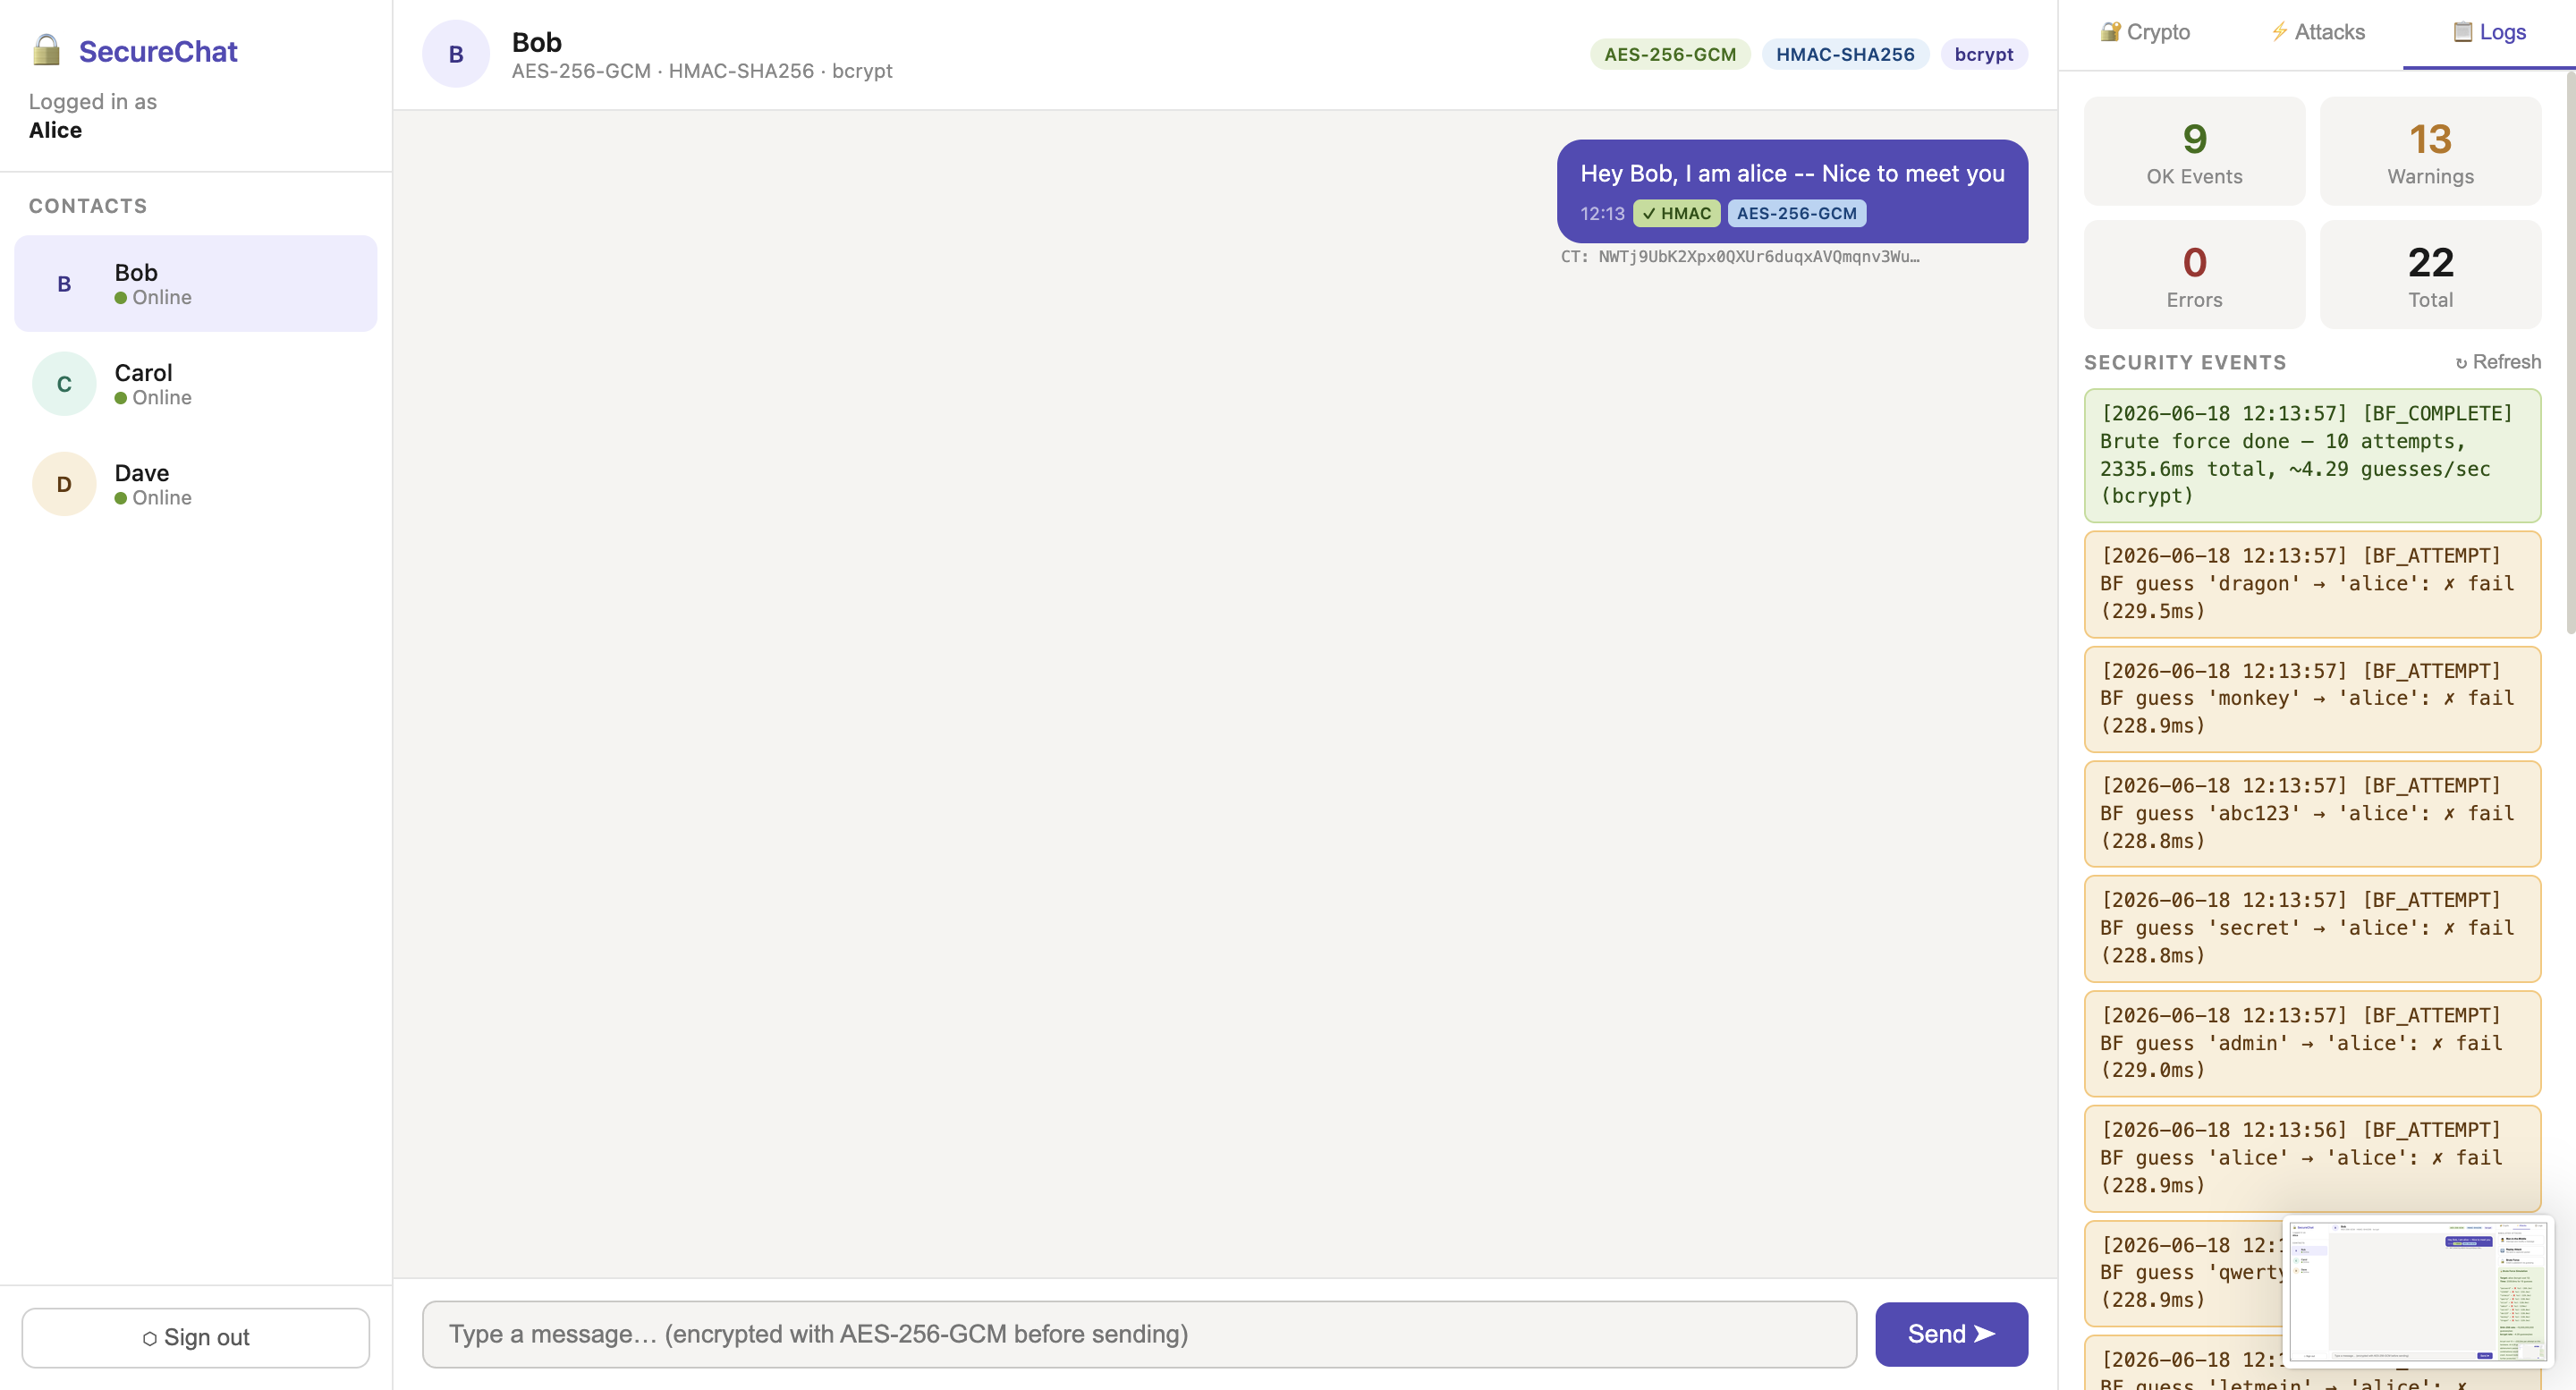
\includegraphics[width=\columnwidth]{sc_logs.png}
    \caption{The live log viewer after a brute-force simulation. The counters at the top summarise the session (9 OK events, 13 warnings, 0 errors, 22 total) and the scrollable list below shows each individual event in chronological order.}
    \label{fig:logs}
\end{figure}

\begin{table}[H]
\centering
\caption{Categories of events recorded by the logging subsystem.}
\renewcommand{\arraystretch}{1.15}
\begin{tabular}{ll}
\toprule
\textbf{Event Type} & \textbf{Trigger Condition} \\
\midrule
\texttt{LOGIN\_OK}        & Successful authentication \\
\texttt{LOGIN\_FAIL}      & Wrong password or unknown user \\
\texttt{ACCOUNT\_LOCKED}  & Five consecutive failures \\
\texttt{REGISTER\_OK}     & New account created \\
\texttt{MSG\_ENCRYPTED}   & Outbound message encrypted \\
\texttt{MSG\_DECRYPTED}   & Inbound message decrypted \\
\texttt{DECRYPT\_FAIL}    & HMAC or GCM auth-tag mismatch \\
\texttt{MITM\_ATTEMPT}    & MITM simulation triggered \\
\texttt{MITM\_DETECTED}   & Tampering caught by HMAC \\
\texttt{REPLAY\_ATTEMPT}  & Replay simulation triggered \\
\texttt{REPLAY\_DETECTED} & Duplicate nonce rejected \\
\texttt{BF\_ATTEMPT}      & Single brute-force guess \\
\texttt{BF\_COMPLETE}     & Brute-force run finished \\
\texttt{LOGOUT}           & User session closed \\
\bottomrule
\end{tabular}
\label{tab:events}
\end{table}

The log shown in Figure~\ref{fig:logs} contains the trail of a brute-force run: each of the ten guesses appears as a \texttt{BF\_ATTEMPT} entry with the guess, the target username, the outcome, and the elapsed time. The session summary at the top --- ``Brute force done --- 10 attempts, 2335.6ms total, $\sim$4.29 guesses/sec (bcrypt)'' --- is itself logged as a \texttt{BF\_COMPLETE} event. This level of detail would in a real deployment be the principal evidence used to detect an ongoing attack.

% ─── IX. Results and Evaluation ──────────────────────────────────────────────
\section{Results and Evaluation}
\label{sec:results}

\subsection{Functional Correctness}
All six homework requirements were implemented and verified in live testing. Table~\ref{tab:checklist} summarises the mapping from each requirement to its implementation location and verification status.

\begin{table}[H]
\centering
\caption{Mapping of homework requirements to implementation.}
\renewcommand{\arraystretch}{1.15}
\begin{tabular}{p{0.36\columnwidth}p{0.32\columnwidth}p{0.18\columnwidth}}
\toprule
\textbf{Requirement} & \textbf{Implementation} & \textbf{Verified} \\
\midrule
User registration \& login    & bcrypt + session token    & Yes \\
Secure password storage       & bcrypt cost 12            & Yes \\
Session handling              & 256-bit CSPRNG token      & Yes \\
Symmetric encryption          & AES-256-GCM               & Yes \\
No hardcoded keys             & PBKDF2-SHA256 derivation  & Yes \\
Message integrity             & HMAC-SHA256 + GCM tag     & Yes \\
MITM attack simulation        & \texttt{/api/attack/mitm} & Yes \\
Replay attack simulation      & \texttt{/api/attack/replay} & Yes \\
Brute-force simulation        & \texttt{/api/attack/bruteforce} & Yes \\
Login attempt logging         & File + UI log             & Yes \\
Encryption event logging      & File + UI log             & Yes \\
Failed-decryption logging     & \texttt{DECRYPT\_FAIL}    & Yes \\
Web user interface            & Flask + SocketIO + JS     & Yes \\
\bottomrule
\end{tabular}
\label{tab:checklist}
\end{table}

\subsection{Attack Detection Results}
Each attack simulation was run multiple times against a fresh deployment. The result was the same in every run: all three attacks were detected by the appropriate defensive layer with no false negatives.

\begin{table}[H]
\centering
\caption{Detection outcomes across attack simulations.}
\renewcommand{\arraystretch}{1.15}
\begin{tabular}{lll}
\toprule
\textbf{Attack}      & \textbf{Defence}              & \textbf{Outcome} \\
\midrule
MITM (bit-flip)      & HMAC-SHA256 + GCM tag         & Blocked, every run \\
Replay (re-send)     & Nonce ledger lookup           & Blocked, every run \\
Brute force (10 PW)  & bcrypt cost 12 + lockout      & Mitigated, every run \\
\bottomrule
\end{tabular}
\label{tab:results}
\end{table}

\subsection{Measured Performance}
On the development machine, key derivation via PBKDF2 (100{,}000 iterations) took an average of 152\,ms per call. Because keys are derived once per conversation pair rather than once per message, this overhead is invisible to the user. bcrypt verification at cost 12 averaged 233\,ms per attempt, which is the dominant cost of any login. AES-GCM encryption and HMAC computation together account for less than 1\,ms per message, so the throughput of the messaging path is bounded by network and rendering, not by cryptography.

\subsection{Security Design Quality}
Beyond the literal requirements, a number of design choices were made to bring the implementation closer to professional practice:

\begin{itemize}
    \item No secret value is embedded as a literal string anywhere in the source.
    \item Encryption and HMAC use independently derived keys, so a compromise of one does not weaken the other.
    \item IVs are drawn from \texttt{os.urandom} for every single message.
    \item Session tokens use \texttt{secrets.token\_hex}, which is the recommended CSPRNG-backed API in modern Python.
    \item HMAC comparisons use \texttt{hmac.compare\_digest} to prevent timing side-channels.
    \item Nonce registration occurs at send time, not at receive time, which means replay detection is guaranteed even if the message has not yet been delivered.
    \item Failed-attempt counters are checked before bcrypt verification, removing any timing oracle on locked accounts.
\end{itemize}

% ─── X. Limitations ───────────────────────────────────────────────────────────
\section{Limitations and Future Work}

The system as it stands has several deliberate limitations that follow from its scope as a homework demonstration.

The encryption is server-mediated: the server can in principle decrypt any message because it holds the derivation material. A more advanced design would use Diffie-Hellman or X25519 key exchange so that only the endpoints hold the keys, and the server sees nothing but opaque ciphertext. This would shift the system from ``server-trusted'' to ``end-to-end encrypted'' in the strict sense.

Storage is in-memory: a restart loses all users and messages. Adding SQLite or PostgreSQL persistence is a straightforward extension and would not change any of the cryptographic logic.

Transport is over plain HTTP for local testing. In a real deployment, TLS would carry the already-encrypted payload, providing an outer protective layer and protecting metadata such as timestamps and recipient names.

Finally, the seen-nonce set grows unboundedly. A production system would either bind nonces to a time window and prune older entries, or replace the set with a Bloom filter to bound memory at the cost of accepting a small false-positive rate.

% ─── XI. Conclusion ───────────────────────────────────────────────────────────
\section{Conclusion}
\label{sec:conclusion}

This project set out to build a messaging system whose security properties could not only be claimed in writing but inspected in operation. The combination of AES-256-GCM, HMAC-SHA256, bcrypt password storage, and a per-message nonce ledger produced a system that resists the three classes of attack covered in the course material: ciphertext tampering, packet replay, and password guessing. Each defence was demonstrated against a working attack simulation in the same application, and each defence held in every test run.

The exercise reinforced several lessons that often get lost in textbook discussion. First, layered defences matter: the HMAC layer is technically redundant against a correct AES-GCM implementation, but it gives the system a second line of protection and makes the integrity check visible to the user. Second, performance numbers matter: the deliberately slow bcrypt verification is precisely what makes password guessing impractical, and choosing the cost factor is a real engineering decision rather than an afterthought. Third, observability matters: the logging system is what would actually let an operator notice that an attack was in progress, and building it in from the start is far easier than retro-fitting it later.

The result is a small but complete application that meets the homework requirements and provides a base for the more advanced extensions outlined above.

% ─── References ──────────────────────────────────────────────────────────────
\begin{thebibliography}{9}

\bibitem{stallings2017}
W. Stallings,
\textit{Cryptography and Network Security: Principles and Practice}, 7th ed.
Pearson, 2017.

\bibitem{nist_aes}
National Institute of Standards and Technology,
``Recommendation for Block Cipher Modes of Operation: Galois/Counter Mode (GCM),''
NIST Special Publication 800-38D, 2007.

\bibitem{rfc2104}
H. Krawczyk, M. Bellare, and R. Canetti,
``HMAC: Keyed-Hashing for Message Authentication,''
IETF RFC 2104, 1997.

\bibitem{bcrypt1999}
N. Provos and D. Mazi\`eres,
``A Future-Adaptable Password Scheme,''
in \textit{Proc. USENIX Annual Technical Conference}, 1999, pp. 81--91.

\bibitem{rfc8018}
K. Moriarty, B. Kaliski, and A. Rusch,
``PKCS \#5: Password-Based Cryptography Specification Version 2.1,''
IETF RFC 8018, 2017.

\bibitem{kocher1996timing}
P. C. Kocher,
``Timing Attacks on Implementations of Diffie-Hellman, RSA, DSS, and Other Systems,''
in \textit{Advances in Cryptology --- CRYPTO '96}, Springer, 1996, pp. 104--113.

\bibitem{python_cryptography}
Python Cryptographic Authority,
``cryptography --- Cryptographic Recipes and Primitives for Python,''
\url{https://cryptography.io}, accessed June 2026.

\bibitem{flask}
A. Ronacher,
``Flask: A Lightweight WSGI Web Application Framework,''
\url{https://flask.palletsprojects.com}, accessed June 2026.

\end{thebibliography}

\end{document}